% voodoo for arXiv scripts
\pdfoutput=1
\documentclass[aps,prd,twocolumn,superscriptaddress,preprintnumbers,floatfix,nofootinbib]{revtex4-2}

\usepackage{graphicx}  
\usepackage{natbib} 
\usepackage{amsmath}
%\usepackage{mdwlist}
%\usepackage[caption=false]{subfig}
%\usepackage{siunitx}
%\usepackage{placeins}
\usepackage{color}
%\usepackage{standalone}
\usepackage{dcolumn}
\usepackage{tensor}
\usepackage{bm}
\usepackage{makecell}
%\usepackage{MnSymbol}
\usepackage[T1]{fontenc}
\usepackage[utf8]{inputenc}
\usepackage{microtype}
\usepackage{etoolbox}
\usepackage{amssymb}
\usepackage{mathrsfs}
\usepackage{accents}
\usepackage[normalem]{ulem}
\usepackage[table,dvipsnames]{xcolor}
\usepackage[colorlinks,urlcolor=NavyBlue,citecolor=NavyBlue,linkcolor=NavyBlue,pdfusetitle]{hyperref}
\usepackage[all]{hypcap}
\usepackage[inline,shortlabels]{enumitem}
\usepackage{braket}
\usepackage{booktabs}
\usepackage{ulem}

\usepackage{array}
\usepackage{diagbox}
\usepackage{color}
\usepackage{colortbl}
\usepackage{hhline}
\usepackage{multirow}

\graphicspath{{./}{figs/}}

\newcommand{\nn}{\nonumber}
\newcommand{\NR}{\text{NR}}
\newcommand{\mmt}[1]{\textcolor{cyan}{#1}}
\newcommand{\lorena}[1]{\textcolor{RoyalPurple}{#1}}
\newcommand{\dimitra}[1]{\textcolor{teal}{#1}}

%%%%%%%%%%%%%%%%%%%%%%%%%%%%%%%%%%%%%%%%%%%%%%%%%%%%%%%%%%%%
%% Author information
%%%%%%%%%%%%%%%%%%%%%%%%%%%%%%%%%%%%%%%%%%%%%%%%%%%%%%%%%%%%


%\usepackage{orcidlink}

\newcommand{\MST}{\affiliation{Institute of Multi-messenger Astrophysics and Cosmology \& Physics Department, 
		Missouri University of Science and Technology, Rolla, MO 65409, USA}}
\newcommand{\OleMiss}{\affiliation{Department of Physics and Astronomy,
		University of Mississippi, University, Mississippi 38677, USA}}
\newcommand{\Torino}{\affiliation{Dipartimento di Fisica,
		Università di Torino \& INFN Sezione di Torino, via P. Giuria 1, 10125 Torino, Italy}}
\newcommand{\Tubingen}{\affiliation{Theoretical Astrophysics Department, 
		Eberhard-Karls University of T\"{u}bingen, T\"{u}bingen 72076, Germany}}
\newcommand{\UAB}{\affiliation{Departament de Matem\`{a}tiques,
		Universitat Aut\`{o}noma de Barcelona, 08193 Bellaterra, Spain}}
\newcommand{\UV}{\affiliation{Departament d’Astronomia i Astrof\'{i}sica,
		Universitat de Val\`{e}ncia, Dr. Moliner 50, 46100, Burjassot (Val\`{e}ncia), Spain}}
		
\begin{document}

%Title of paper
\title{Work in Classification}

\author{Simone Albanesi}
%	\orcidlink{0000-0001-7345-4415}}
\email{simone.albanesi@edu.unito.it}
\Torino
\author{Marina Berbel}
%	\orcidlink{0000-0001-6345-1798}}
\email{mberbel@mat.uab.cat}
\UAB
\author{Marco Cavagli\`{a}}
%	\orcidlink{0000-0002-3835-6729}}
\email{cavagliam@mst.edu}
\MST
\author{Lorena \surname{Magaña Zertuche}}
%	\orcidlink{0000-0003-1888-9904}}
\email{lmaganaz@go.olemiss.edu}
\OleMiss
\author{Miquel Miravet-Ten\'{e}s}
%	\orcidlink{0000-0002-8766-1156}}
\email{miquel.miravet@uv.es}
\UV
\author{Dimitra Tseneklidou}
%	\orcidlink{0000-0003-2582-1705}}
\email{dimitra.tseneklidou@uni-tuebingen.de}
\Tubingen
\author{Yanyan Zheng}
%	\orcidlink{0000-0002-5432-1331}}
\email{zytfc@umsystem.edu}
\MST
%\author{Any other?}
%	\orcidlink{}}
%\email{}


% Because hyperref only gets the *last* author, we need to be explicit.
\hypersetup{pdfauthor={LastName et al.}}

\date{\today}

\begin{abstract}

Because of the electromagnetic radiation produced during the merger, compact binary coalescences with neutron stars may result in multi-messenger observations. In order to follow up on the
gravitational-wave signal with electromagnetic telescopes, it is critical to promptly identify the properties of these sources.  This identification must rely on the properties of the progenitor
source, such as the component masses and spins, as determined by low-latency detection pipelines in real time. The output of these pipelines, however, might be biased, which could decrease the
accuracy of parameter recovery. Machine learning algorithms are used to correct this bias. In this work, we revisit this problem and discuss \tocheck{\sout{the implementation of two}} \tocheck{two new implementations} of supervised machine learning algorithms, K-Nearest Neighbors and Random Forest, which are able to predict the presence of a neutron star and post-merger matter remnant in \tocheck{low-latency} compact binary coalescence \tocheck{\sout{more accurately than the low latency infrastructure currently used by LIGO, Virgo, and KAGRA}} \tocheck{searches across different search pipelines and algorithms}. Additionally, we present a novel approach for calculating the Bayesian probabilities for these two metrics. Instead of metric
scores derived from binary machine learning classifiers, our scheme is designed to provide the astronomy community well-defined probabilities. This would deliver a more direct and easily
interpretable product to assist electromagnetic telescopes in deciding whether to follow up on gravitational-wave events in real time.

\end{abstract}


%\maketitle must follow title, authors, abstract, \pacs, and \keywords
\maketitle

%\tableofcontents

% body of paper here - Use proper  commands
% References should be done using the \cite, \ref, and \label commands

\section{Introduction} \label{intro}
%In our introduction we want to start from big picture (LIGO, ML, pipelines)
%and narrow down to what work we are presenting here and why it is important. We
%also describe in which ways it is novel and how it compares to previous works
%like in~\cite{Chatterjee:2019avs}. We may also want to cite~\cite{Sachdev:2020lfd}. 

The first detection of a \ac{GW} signal from a pair of coalescing black holes in 2015 and the first observation of a coalescing binary neutron star system two years later have established \ac{MMA} as
a powerful tool for the exploration of the cosmos~\cite{LIGOScientific:2016aoc,LIGOScientific:2017vwq,LIGOScientific:2018cki}. The third \ac{LVK} catalog of transient \ac{GW} signals
\ac{GWTC3}~\cite{LIGOScientific:2021djp} has shown that \ac{GW} astronomy has entered its mature phase, becoming a true observational branch of astronomy. \ac{MMA} allows scientists to explore
in depth the origin and structure of black holes~\cite{Schmidt:2020ekt,Nitz:2021zwj}, neutron stars~\cite{Lasky:2015uia,Baiotti:2016qnr} and gamma-ray bursts~\cite{Ciolfi:2018tal}, test general
relativity \todo{ref needed here}, probe the fundamental nature of gravity~\cite{Kurpas2022}, and measure the evolution of the
universe~\cite{LIGOScientific:2021sio,LIGOScientific:2021psn,LIGOScientific:2021aug}. \todo{check all the above references, make sure bibliography is complete and up to date}

A wealth of new detections is being amassed to achieve these science goals~\cite{LIGOScientific:2014pky,VIRGO:2014yos}. The rate of detections in \ac{LVK}'s \ac{O4} is close to one per day and
is expected to further increase in the \ac{O5}~\cite{KAGRA:2013rdx}. Over the course of \ac{O4} and the next observing runs, the \ac{LVK} collaboration will analyze hundreds of \ac{BBH} and
dozens of \ac{BNS} and \ac{NSBH} detections, several of which could be \ac{MMA} sources. Among the challenges that this new phase of \ac{GW} astronomy brings is the necessity to coordinate the
activities of \ac{EM} and \ac{GW} observatories in real time. 

One of the most interesting areas of study in \ac{MMA} astronomy is the physics of gravity-matter interaction in \ac{GW} sources. Tidally disrupted matter in an \ac{NSBH} system may form a
high-temperature accretion disk around the \ac{BH} and trigger the creation of a prompt \ac{EM} emission in the form of a short \ac{GRB}. If the system ejecta are unbound, r-process
nucleosynthesis may lead to a \ac{KN}~\cite{Lattimer:1974slx, Li:1998bw, Korobkin:2012uy, Barnes:2013wka, Tanaka:2013ana, Kasen:2014toa}. These phenomena could also arise in \ac{BNS}
post-mergers through the expulsion of neutron-rich material even when tidal forces are weak~\cite{LIGOScientific:2017ync, Arcavi:2017xiz, Coulter:2017wya, Kasliwal:2017ngb, Lipunov:2017dwd,
DES:2017kbs, Tanvir:2017pws}. The presence of a post-merger matter remnant, which results in an \ac{EM} signature or a prompt collapse, is a common factor in all of these scenarios. Determining
the potential of a \ac{GW} source to become an \ac{EM} emitter and enabling coincident observations of these systems by \ac{EM} and \ac{GW} observatories in low latency are crucial for the success
of \ac{MMA}.

The \ac{LVK} employs different matched-filtering pipelines for low-latency \ac{GW} searches~\cite{Sachdev:2020lfd,Nitz:2018rgo,Adams:2015ulm} \todo{add and check references for pipelines and add
spiir}. These searches are based on discrete template banks of \ac{CBC} waveforms that provide, among other parameters, the component masses and the dimensionless (anti-)aligned spins of the
objects along the orbital angular momentum. These parameters can be used to determine the \ac{EM} properties of \ac{GW} candidates in real time through empirical fits of \ac{NR}
simulations~\cite{Foucart:2012nc,Foucart:2018rjc}. Low-latency preliminary alerts of candidate \ac{GW} events in the \ac{O3} included two \ac{EM}-property metrics identifying whether the
\ac{CBC} system contains a \ac{NS}, \hasns, and a post-merger matter remnant, \hasrem. Alerts with similar content continue to be issued in \ac{O4} with a \todo{median?} latency of the order of
one second after the detection of candidate merger events.  Additionally, \ac{LVK}'s \ac{O4} alerts include a measure of the \hasgap\ property, i.e., the likelihood that one of the source
compact objects has a mass in the lower-mass gap region between \ac{NS}s and \ac{BH}s \todo{ref of user guide or other here}.

Classification of \ac{GW} candidate events in low latency poses several challenges as the desire for accuracy contrasts with the desire to issue the information as quickly as possible. The
approach taken by the \ac{LVK} so far has been to use a supervised \ac{KNN}~\cite{Pedregosa:2011ork} \ac{ML} algorithm with input from the detection pipelines and \ac{EOS} models to generate
independent \hasns\ and \hasrem\ binary classification \emph{scores}~\cite{Chatterjee:2019avs}. The \ac{KNN} model is trained on a broad set of synthetic \ac{CBC} signals injected in real
detector noise from the \ac{O2}. The advantage of this scheme relies in the capability of the method to handle the statistical uncertainties of the parameters from the search pipelines and the
non-stationarity of the detectors' power spectral density. This approached allowed for a marked improvement in performance compared to the semi-analytic effective Fisher formalism method that
was deployed in \ac{O2}.

In this work, we revisit the problem of the real-time production of \hasns\ and \hasrem\ \emph{probability} metrics with the aim of further improving the latency and performance of the current
\ac{LVK} \ac{ML}-based scheme~\cite{Chatterjee:2019avs}. In the current implementation, the validity of the classification outcome for an event is assessed through elements of the algorithm's
confusion matrix and its \ac{ROC} curve. For example, given a positive prediction, the \ac{LVK} defines a ``score'' that this prediction is correct as the \ac{TPR} for the given data
set. However, there is no quantity in the algorithm's confusion matrix that defines a probability in the strictest sense. A second limitation of current \hasns\ and \hasrem\ classification
schemas is the fact that the \hasns\ and \hasrem\ labels are treated as independent variables. In reality, the probability of a system being \ac{EM} bright is always smaller than the probability
of the system hosting a \ac{NS}. Therefore, the \hasns\ and \hasrem\ labels cannot be treated as disjoint. In the current \ac{LVK} implementation, this physical condition is data-based rather
than being mathematically defined, i.e., the algorithm potentially allows for violations and the absence of inversions is only checked a posteriori through (coarse) parameter sweeps. One of the
main purposes of this work is to go beyond the above scheme and calculate true \emph{conditional Bayesian probabilities} for \hasns\ and \hasrem. 

To achieve this, we design a new classification scheme and perform a thorough study and comparison of two alternative \ac{ML} algorithms. We first implement a definition for conditional \hasns\
and \hasrem\ metrics that incorporates \emph{ab initio} the physical requirement that a system with a post-merger matter remnant must necessarily contain a \ac{NS}. Then we calculate
\emph{Bayesian probabilities} for \hasns\ and \hasrem. We also implement a marginalization procedure over a set of \ac{EOS} that minimizes possible systematics arising from the use of a single
\ac{EOS}. Finally, test the performance of the scheme and the algorithms on synthetic \ac{O3} signals and confident \ac{GW} detections from the latest \ac{GWTC3} catalog.

The structure of the paper is as follows. Section~\ref{algos} introduces the classification algorithms. Bayesian probabilities for \hasns\ and \hasrem\ and the labeling scheme are defined in
Sec.~\ref{probability}. The data set is described in Sec.~\ref{dataset}. Results and algorithm comparison are reported in Sec.~\ref{results}. Conclusions and future developments are presented in Sec.~\ref{conclusions}.  

%here why ligo wants to classify, alert astronomers, try to improve previous work (KNN) exploring more algo (RF and GP), but present also KNN for direct comparison


\section{Data set\label{dataset}}
\label{sec:dataset}

In our analysis, we employ the same data set as Ref.\ \todo{chatterjee}. This allows us to directly compare the performance of the various algorithms and the new labeling
scheme to the performance of the \ac{KNN} algorithm, which was deployed in the latest \ac{LVK} observing run. 

We train the \ac{KNN} and \ac{RF} algorithms on a broad injection campign where the injections were made in two detector operations from \ac{O2} observing run with synthetic \ac{BNS}, \ac{NSBH}, and \ac{BBH} signals. The injection population contains uniform/loguniform distribution of the masses, with both aligned and isotropic distributions of spins and was used primarily for the spacetime volume sensitivity analysis for the GstLAL search in Abbott et al. \todo{cite this paper from GstLAL}(2019b). Further details on the injection waveforms and quantitive info of masses and spins can be found in \todo{chatterjee}. The \ac{CBC} signals are recovered with one of the standard search \ac{LVK} pipelines, the GstLAL pipeline. It a stream-based matched filtering algorithm capable of detecting \ac{GW} signals within seconds of their arrival on Earth \todo{cite Messick, Tsukada, Ewing}. Because of the signal strength and reduced detector senstivity, not all injections were found by the search. The injections that were found, along with its pipeline recovered counterpart, were used to make the dataset. Each recovered triggers is assigned a false-alarm rate (FAR) based on the frequency of background triggers and quntifies the significance of the detection. In order to select more sigificant recovered triggers, we imposed a cut of $FAR <= 1/month$ in this work.  

The dimension of the data set is determined by the number of signals recovered by the pipeline after proper cuts are applied ($\sim2.0X10^5$). The intrinsic source properties of the merger: primary and secondary masses and spins ({$m_1$,$m_2$,$\chi_1$,$\chi_2$}) and the recovered signal to noise ratio (SNR) were used for training RF and KNN algorithms.


%for ML we need data, we use injections in O2. Usually the labels of NS and REM were put in this way. Then we do multilabel with that in this other way.
%In particular to classify the REM we use 23 eos, that ligo chooses to be candidates covering wide parameter space (REF). So we have an algo for every of them. Probabilities are finally combined with weighted average by bayes factor (ref).

%\section{Improving Binary Classification through ML}
\label{sec:ML_concept}
In this section we may want to expand on the idea of using classification itself.
We should mention which algorithms we attempted to use and why they did not
work. Then we can talk more in detail about the ones that did work in the
following subsections.
%improving? that's not explaining the algo. I would call the section "Algorithms and results" or something similar
\section{Classification Algorithms}
\subsection{K-Nearest Neighbors (KNN)}

One of the non-parametric algorithms we have used for classification is the \texttt{KNeighborsClassifier} (KNN). This algorithm assumes that similar things are near to each other.  It captures the idea of similarity by computing the distance between points in a graph.  It is also a lazy learning algorithm, because it does not have a training phase, it uses all the data for training while classification -the dataset is stored and at the time of classification, it acts on the dataset. 

The workflow of the KNN algorithm is the following: first,  after splitting the data into training and testing sets, we need to select the number of neighbors, $K$,  which can be any integer.  Then, for each point of the testing dataset we compute the distance between the point and each row of the training data with a chosen metric (\texttt{euclidean, manhattan, chebysev, mahalanobis}), and we sort the points in ascending order based on the distance value.  By choosing the top $K$ neighbors from the sorted array, we assign a class to the test point, which is the most frequent class of the chosen neighbors.

\section{Random Forest (RF)}

A RF is an ensemble of decision trees. One of its major strengths is that every train trains and classifies independently from the rest, while the RF classification joints all the results and assign as category the mode from the trees. The probability of belonging to a category is therefore straightforward, being the number of trees that chose it divided by the total number of trees. Notice that the training and evaluation of a RF can be accelerated by parallelization, as computations inside each tree are independent from the rest.

The training of a RF is usually done with bootstrap, a technique that assigns a random subset of the training dataset to each tree. This prevents overfitting as every individual classifier is not exposed to the same data, and encourages pattern recognition by studying the same data from different subsets. Every decision tree is composed by nodes, where data its splitted until the different categories are separated. At each node, a subset of the features of the data is selected along threshold values that maximize the information gain at the separation. The binary splitting at each node gives the tree its name, as it can be visualized as roots going deeper at separations.

We use the RK implementation in scikitlearn [REF AND DETAILS]. The main hyperparameters to tune in this module are the number of trees, the maximum depth allowed and the information gain criteria used at splitting (two are offered). We have observed that the maximum number of features to be considered in a node can be kept fix as the square root of the total number of features. Given that the aiming of this work is to improve the current low latency classification, the model once trained can occupy a restricted amount of memory. Therefore before searching the optimum hyperparameters for our dataset, we restrict those which make heavier models: the number of trees and their depth. We set to 100 the maximum number of trees the forest may have, and 25 their possible maximum depth.

For the RF we use events with 5 features: the two masses, their corresponding spins and the SNR of the detection. In the tuning of the hyperparameters we measure the performance  by its score: the number of events correctly classified against the total number of events in the testing dataset, if threshold is taken as 0.5. As all categories are balanced, this approach is enough to roughly compare models. The best model found achieves a score of $whatever$ using $number$ of trees, $number$ maximum depth and $name$ criteria for the information gain.

INFORMATION TO SAY, JUST HERE AND NOT WELL WRITTEN:

For the 23 EoS we try a crossvalidation with:

trees in the forest = [10, 30, 50, 80, 100, 300]  (more trees take too much memory)
criterion = ‘entropy’    (in all tests, criterion ‘gini’ gives very similar results)

max\_features = ‘sqrt’ (in all tests, using a portion of the features instead of all of them in each node gives better results)

max\_depth = [15, 25, 35, 45, None] (we would prefer more shallow trees)

Using the complete dataset, and not Sushant partitions, Use  first 30% of the rows to test, rest 70% of the rows to train

We obtain the following:

% Please add the following required packages to your document preamble:
% \usepackage{booktabs}
\begin{table}[]
\centering
\begin{tabular}{@{}cccccccccccc@{}}
\toprule
\multicolumn{1}{l}{}               & \multicolumn{5}{c}{Best}                                                                                                                                                                  & \multicolumn{5}{c}{Second best}                                                                                                                                                           & \multicolumn{1}{l}{}                 \\ \midrule
\multicolumn{1}{|c|}{\textbf{EOS}} & \multicolumn{1}{c|}{\textbf{Trees}} &
    \multicolumn{1}{c|}{\textbf{Depth}} & \multicolumn{1}{c|}{\textbf{Score}} &
    \multicolumn{1}{c|}{\textbf{MB}} & \multicolumn{1}{c|}{\textbf{MB (c)}} &
    \multicolumn{1}{c|}{\textbf{Trees}} & \multicolumn{1}{c|}{\textbf{Depth}} &
    \multicolumn{1}{c|}{\textbf{Score}} & \multicolumn{1}{c|}{\textbf{MB}} &
    \multicolumn{1}{c|}{\textbf{MB (c)}} & \multicolumn{1}{c|}{\textbf{$\Delta$ score}} \\ \midrule
\multicolumn{1}{|c|}{APR4\_BB}     & \multicolumn{1}{c|}{300}            & \multicolumn{1}{c|}{15}             & \multicolumn{1}{c|}{0.9683018}      & \multicolumn{1}{c|}{94.7}        & \multicolumn{1}{c|}{19.7}            & \multicolumn{1}{c|}{50}             & \multicolumn{1}{c|}{15}             & \multicolumn{1}{c|}{0.9682683}      & \multicolumn{1}{c|}{15.7}        & \multicolumn{1}{c|}{3.3}             & \multicolumn{1}{c|}{3.35e-5}         \\ \midrule
\multicolumn{1}{|c|}{BHF\_BBB2}    & \multicolumn{1}{c|}{80}             & \multicolumn{1}{c|}{15}             & \multicolumn{1}{c|}{0.9685127}      & \multicolumn{1}{c|}{24.4}        & \multicolumn{1}{c|}{5.1}             & \multicolumn{1}{c|}{300}            & \multicolumn{1}{c|}{15}             & \multicolumn{1}{c|}{0.9684611}      & \multicolumn{1}{c|}{91.6}        & \multicolumn{1}{c|}{19.2}            & \multicolumn{1}{c|}{5.16e-5}         \\ \midrule
\multicolumn{1}{|c|}{H4}           & \multicolumn{1}{c|}{80}             & \multicolumn{1}{c|}{15}             & \multicolumn{1}{c|}{0.9618587}      & \multicolumn{1}{c|}{29.6}        & \multicolumn{1}{c|}{6.1}             & \multicolumn{1}{c|}{300}            & \multicolumn{1}{c|}{15}             & \multicolumn{1}{c|}{0.9617395}      & \multicolumn{1}{c|}{111.4}       & \multicolumn{1}{c|}{23}              & \multicolumn{1}{c|}{1.19e-4}         \\ \midrule
\multicolumn{1}{|c|}{HQC18}        & \multicolumn{1}{c|}{300}            & \multicolumn{1}{c|}{15}             & \multicolumn{1}{c|}{0.9673755}      & \multicolumn{1}{c|}{93.7}        & \multicolumn{1}{c|}{19.6}            & \multicolumn{1}{c|}{100}            & \multicolumn{1}{c|}{15}             & \multicolumn{1}{c|}{0.9670695}      & \multicolumn{1}{c|}{31.3}        & \multicolumn{1}{c|}{6.6}             & \multicolumn{1}{c|}{3.06e-4}         \\ \midrule
\multicolumn{1}{|c|}{KDE0V}        & \multicolumn{1}{c|}{300}            & \multicolumn{1}{c|}{15}             & \multicolumn{1}{c|}{0.9673295}      & \multicolumn{1}{c|}{92.0}        & \multicolumn{1}{c|}{19.3}            & \multicolumn{1}{c|}{80}             & \multicolumn{1}{c|}{15}             & \multicolumn{1}{c|}{0.9671236}      & \multicolumn{1}{c|}{24.5}        & \multicolumn{1}{c|}{5.1}             & \multicolumn{1}{c|}{2.06e-4}         \\ \midrule
\multicolumn{1}{|c|}{KDE0V1}       & \multicolumn{1}{c|}{100}            & \multicolumn{1}{c|}{15}             & \multicolumn{1}{c|}{0.96704954}     & \multicolumn{1}{c|}{30.9}        & \multicolumn{1}{c|}{6.5}             & \multicolumn{1}{c|}{80}             & \multicolumn{1}{c|}{15}             & \multicolumn{1}{c|}{0.96701525}     & \multicolumn{1}{c|}{24.5}        & \multicolumn{1}{c|}{5.2}             & \multicolumn{1}{c|}{3.43e-5}         \\ \midrule
\multicolumn{1}{|c|}{MPA1}         & \multicolumn{1}{c|}{80}             & \multicolumn{1}{c|}{15}             & \multicolumn{1}{c|}{0.96601225}     & \multicolumn{1}{c|}{27.2}        & \multicolumn{1}{c|}{5.6}             & \multicolumn{1}{c|}{300}            & \multicolumn{1}{c|}{15}             & \multicolumn{1}{c|}{0.96593032}     & \multicolumn{1}{c|}{102.1}       & \multicolumn{1}{c|}{21.2}            & \multicolumn{1}{c|}{8.19e-5}         \\ \midrule
\multicolumn{1}{|c|}{MS1\_PP}      & \multicolumn{1}{c|}{300}            & \multicolumn{1}{c|}{15}             & \multicolumn{1}{c|}{0.96563534}     & \multicolumn{1}{c|}{113.5}       & \multicolumn{1}{c|}{23.2}            & \multicolumn{1}{c|}{80}             & \multicolumn{1}{c|}{15}             & \multicolumn{1}{c|}{0.96552063}     & \multicolumn{1}{c|}{30.2}        & \multicolumn{1}{c|}{6.2}             & \multicolumn{1}{c|}{1.15e-4}         \\ \midrule
\multicolumn{1}{|c|}{MS1B\_PP}     & \multicolumn{1}{c|}{300}            & \multicolumn{1}{c|}{15}             & \multicolumn{1}{c|}{0.96555340}     & \multicolumn{1}{c|}{114.2}       & \multicolumn{1}{c|}{23.3}            & \multicolumn{1}{c|}{100}            & \multicolumn{1}{c|}{15}             & \multicolumn{1}{c|}{0.96535675}     & \multicolumn{1}{c|}{38.0}        & \multicolumn{1}{c|}{7.8}             & \multicolumn{1}{c|}{1.97e-4}         \\ \midrule
\multicolumn{1}{|c|}{RS}           & \multicolumn{1}{c|}{300}            & \multicolumn{1}{c|}{15}             & \multicolumn{1}{c|}{0.96447350}     & \multicolumn{1}{c|}{103.8}       & \multicolumn{1}{c|}{21.6}            & \multicolumn{1}{c|}{80}             & \multicolumn{1}{c|}{15}             & \multicolumn{1}{c|}{0.96423756}     & \multicolumn{1}{c|}{27.6}        & \multicolumn{1}{c|}{5.7}             & \multicolumn{1}{c|}{2.36e-4}         \\ \midrule
\multicolumn{1}{|c|}{SK255}        & \multicolumn{1}{c|}{300}            & \multicolumn{1}{c|}{15}             & \multicolumn{1}{c|}{0.96472405}     & \multicolumn{1}{c|}{105.8}       & \multicolumn{1}{c|}{22.0}            & \multicolumn{1}{c|}{100}            & \multicolumn{1}{c|}{15}             & \multicolumn{1}{c|}{0.9643546}      & \multicolumn{1}{c|}{35.5}        & \multicolumn{1}{c|}{7.4}             & \multicolumn{1}{c|}{3.69e-4}         \\ \bottomrule
\end{tabular}
\caption{table1 comparison forests}
\label{tab:RF1}
\end{table}


% Please add the following required packages to your document preamble:
% \usepackage{booktabs}
\begin{table}[]
\centering
\begin{tabular}{@{}|c|ccccc|ccccc|c|@{}}
\toprule
\multicolumn{1}{|l|}{} & \multicolumn{5}{c|}{Best}                                                                                                                                            & \multicolumn{5}{c|}{Second Best}                                                                                                                                     &                 \\ \midrule
\textbf{EOS}           & \multicolumn{1}{c|}{\textbf{Trees}} &
    \multicolumn{1}{c|}{\textbf{Depth}} & \multicolumn{1}{c|}{\textbf{Score}} &
    \multicolumn{1}{c|}{\textbf{MB}} & \textbf{MB (c)} &
    \multicolumn{1}{c|}{\textbf{Trees}} & \multicolumn{1}{c|}{\textbf{Depth}} &
    \multicolumn{1}{c|}{\textbf{Score}} & \multicolumn{1}{c|}{\textbf{MB}} &
    \textbf{MB (c)} & \textbf{$\Delta$ score} \\ \midrule
SK272                  & \multicolumn{1}{c|}{300}            & \multicolumn{1}{c|}{15}             & \multicolumn{1}{c|}{0.96401816}     & \multicolumn{1}{c|}{109.0}       & 22.6            & \multicolumn{1}{c|}{100}            & \multicolumn{1}{c|}{15}             & \multicolumn{1}{c|}{0.96381927}     & \multicolumn{1}{c|}{36.4}        & 7.5             & 1.99e-4         \\ \midrule
SKI2                   & \multicolumn{1}{c|}{50}             & \multicolumn{1}{c|}{15}             & \multicolumn{1}{c|}{0.96242338}     & \multicolumn{1}{c|}{18.8}        & 3.9             & \multicolumn{1}{c|}{300}            & \multicolumn{1}{c|}{15}             & \multicolumn{1}{c|}{0.96233966}     & \multicolumn{1}{c|}{112.8}       & 23.2            & 8.37e-5         \\ \midrule
SKI3                   & \multicolumn{1}{c|}{50}             & \multicolumn{1}{c|}{15}             & \multicolumn{1}{c|}{0.96174537}     & \multicolumn{1}{c|}{19.0}        & 3.9             & \multicolumn{1}{c|}{100}            & \multicolumn{1}{c|}{15}             & \multicolumn{1}{c|}{0.96167916}     & \multicolumn{1}{c|}{38.1}        & 7.8             & 6.62e-5         \\ \midrule
SKI4                   & \multicolumn{1}{c|}{300}            & \multicolumn{1}{c|}{15}             & \multicolumn{1}{c|}{0.96598969}     & \multicolumn{1}{c|}{100.6}       & 20.9            & \multicolumn{1}{c|}{30}             & \multicolumn{1}{c|}{15}             & \multicolumn{1}{c|}{0.96590604}     & \multicolumn{1}{c|}{9.8}         & 2.1             & 8.37e-5         \\ \midrule
SKI5                   & \multicolumn{1}{c|}{100}            & \multicolumn{1}{c|}{15}             & \multicolumn{1}{c|}{0.96343381}     & \multicolumn{1}{c|}{38.2}        & 7.8             & \multicolumn{1}{c|}{80}             & \multicolumn{1}{c|}{15}             & \multicolumn{1}{c|}{0.96331793}     & \multicolumn{1}{c|}{30.4}        & 6.2             & 1.16e-4         \\ \midrule
SKI6                   & \multicolumn{1}{c|}{300}            & \multicolumn{1}{c|}{15}             & \multicolumn{1}{c|}{0.96586928}     & \multicolumn{1}{c|}{101.7}       & 21.1            & \multicolumn{1}{c|}{30}             & \multicolumn{1}{c|}{15}             & \multicolumn{1}{c|}{0.96565242}     & \multicolumn{1}{c|}{10.0}        & 2.1             & 2.17e-4         \\ \midrule
SKMP                   & \multicolumn{1}{c|}{300}            & \multicolumn{1}{c|}{15}             & \multicolumn{1}{c|}{0.96544567}     & \multicolumn{1}{c|}{100.2}       & 20.9            & \multicolumn{1}{c|}{80}             & \multicolumn{1}{c|}{15}             & \multicolumn{1}{c|}{0.96527695}     & \multicolumn{1}{c|}{26.9}        & 5.6             & 1.69e-4         \\ \midrule
SKOP                   & \multicolumn{1}{c|}{100}            & \multicolumn{1}{c|}{15}             & \multicolumn{1}{c|}{0.96610459}     & \multicolumn{1}{c|}{32.3}        & 6.8             & \multicolumn{1}{c|}{300}            & \multicolumn{1}{c|}{15}             & \multicolumn{1}{c|}{0.96603605}     & \multicolumn{1}{c|}{96.2}        & 20.1            & 6.85e-5         \\ \midrule
SLy                    & \multicolumn{1}{c|}{80}             & \multicolumn{1}{c|}{15}             & \multicolumn{1}{c|}{0.96728884}     & \multicolumn{1}{c|}{25.3}        & 5.3             & \multicolumn{1}{c|}{300}            & \multicolumn{1}{c|}{15}             & \multicolumn{1}{c|}{0.96720392}     & \multicolumn{1}{c|}{95.2}        & 19.9            & 8.49e-5         \\ \midrule
SLY2                   & \multicolumn{1}{c|}{100}            & \multicolumn{1}{c|}{15}             & \multicolumn{1}{c|}{0.96745868}     & \multicolumn{1}{c|}{31.8}        & 6.6             & \multicolumn{1}{c|}{80}             & \multicolumn{1}{c|}{15}             & \multicolumn{1}{c|}{0.96722091}     & \multicolumn{1}{c|}{25.4}        & 5.3             & 2.38e-4         \\ \midrule
SLY9                   & \multicolumn{1}{c|}{300}            & \multicolumn{1}{c|}{15}             & \multicolumn{1}{c|}{0.96605993}     & \multicolumn{1}{c|}{101.6}       & 21.1            & \multicolumn{1}{c|}{100}            & \multicolumn{1}{c|}{15}             & \multicolumn{1}{c|}{0.96590909}     & \multicolumn{1}{c|}{34.1}        & 7.1             & 1.51e-4         \\ \midrule
SLY230A                & \multicolumn{1}{c|}{300}            & \multicolumn{1}{c|}{15}             & \multicolumn{1}{c|}{0.96714915}     & \multicolumn{1}{c|}{95.5}        & 20.0            & \multicolumn{1}{c|}{100}            & \multicolumn{1}{c|}{15}             & \multicolumn{1}{c|}{0.96689580}     & \multicolumn{1}{c|}{31.9}        & 6.7             & 2.53e-4         \\ \bottomrule
\end{tabular}
\caption{table2 RF comparison}
\label{tab:RF2}
\end{table}



And therefore we select 50 trees, 15 depth for all EoS and present the results with that.



\section{Results}

In order to decide which method gives a better performance in classifying this kind of events, we can apply them over testing data and finally do a comparison between both. A way to see how data is classified we can construct histograms where the number of events that are classified with a label (\texttt{HasNS/HasRemnant}) \texttt{True} or \texttt{False} will change with a given threshold of the probability. For an algorithm with perfect performance, all the events with label \texttt{True (False)} should be at \textit{p}(\texttt{label}) = 1 (\textit{p}(\texttt{label}) = 0).

Another way to check the algorithm's performance is by building the so-called \textit{Receiver Operating Characteristic (ROC) Curve}. They show the variation of the true-positive rate (or efficiency) with the false-positive rate given a certain threshold for the probability. An algorithm with a proper performance will give a steeper ROC curve, or in other words, will have a higher eficiency with a lower false-positive rate.  


In the ROC curves that we will present in the following subsections, we highlight three reference EoS in color, from which we show results in more detail. We select BHF\_BBB2 because is the model that give the lowest maximum mass, MS1\_PP as the model with the bigger maximum mass, and we also include SLy because is the most accepted EoS for NS modeling (reference), and is the one that was used in the injections that are our dataset.

Here are the results for both methods:
\subsection{KNN Results}

%\mmt{We are only using 5 features, the independent variables: 
%\begin{equation*}
	%\big[m_1,m_2,\chi_1,\chi_2, \rm{SNR}\big]\,.
%\end{equation*}}

\subsubsection{\mmt{Has NS}}
\mmt{The metric we use to compute the distance between neighbors is the \textit{Manhattan} metric (or the Minkowski's $L1$ distance),  which is the distance between two points measured along axes at right angles. Having $p_1(x_1,y_1)$ and $p_2(x_2,y_2)$ the distance will be}
\begin{equation}
	d = |x_1-x_2|+|y_1-y_2|\,.
\end{equation}

\mmt{Moreover, the points are weighted uniformly.  After applying cross-validation,  we get that the optimal number of neighbors is $K_{\rm NS} = 10$, with a mean score $\rm{s_m} = 0:9718355224352762$ and a testing score  $\rm{s_t} = 0.9723828730478842$.} 

%\begin{figure}
%    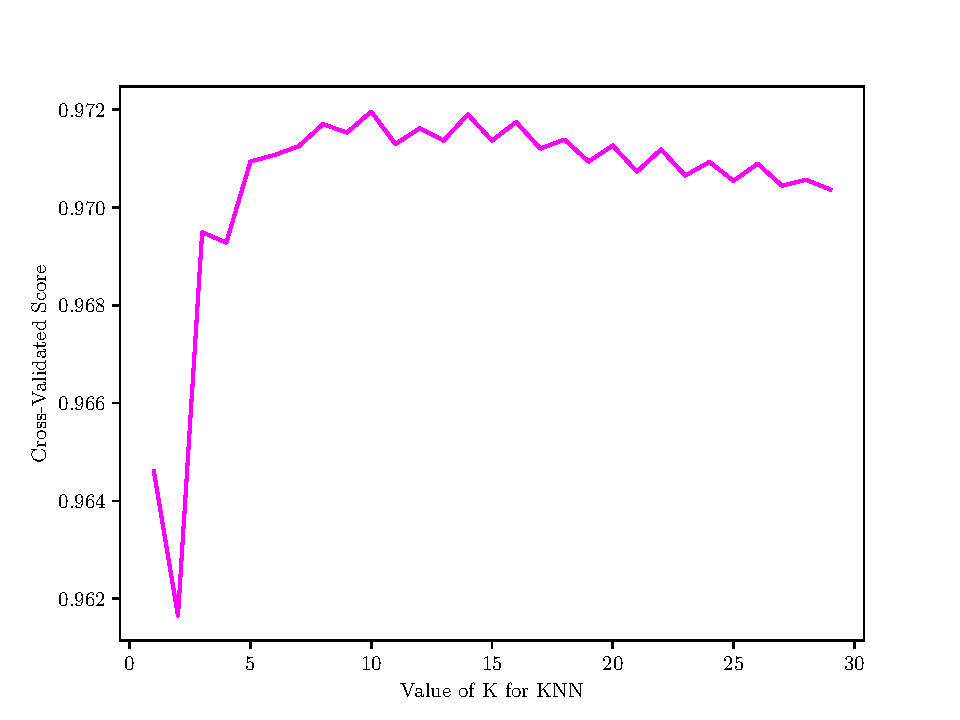
\includegraphics[width = 0.4\textwidth]{CrossValK.pdf}
%    \caption{Score of our KNN model as a function of the number of neighbors. We are considering \textit{HasNS}.}
%    \label{fig:crossvalK}
%\end{figure}
    
\begin{figure}
    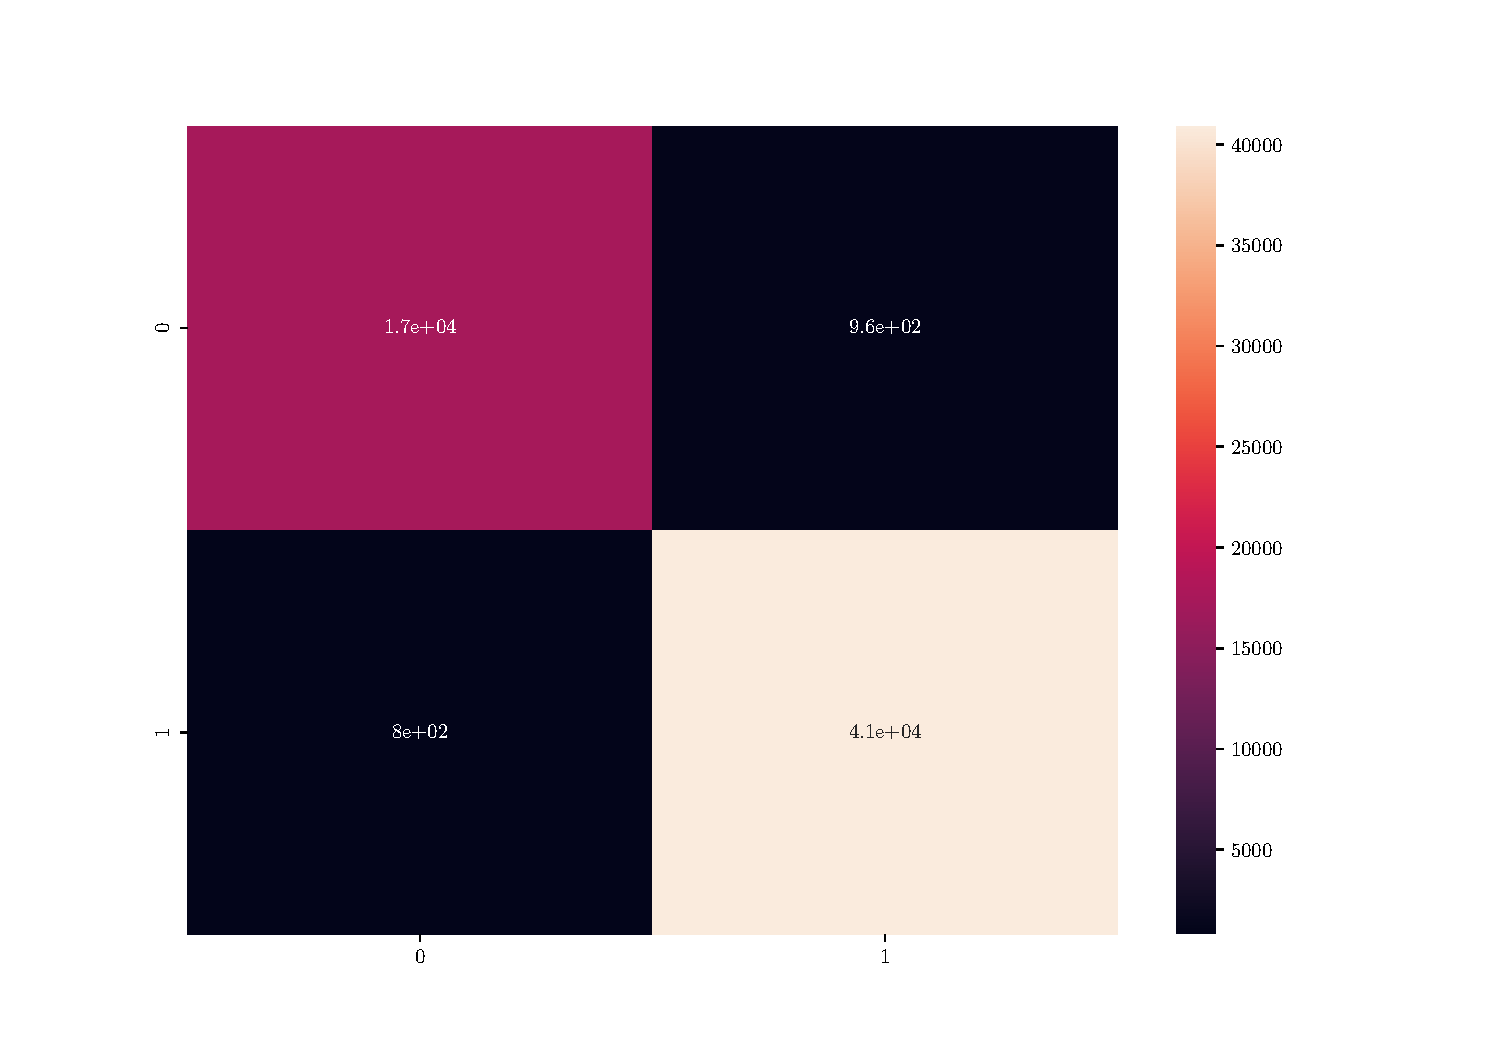
\includegraphics[width=0.45\textwidth]{figs/conf_matrix_NS.pdf}
    \caption{Confusion matrix for our model for \textit{HasNS}, using the independent recovered values. }
    \label{fig:confmat}
\end{figure}

\begin{figure}
    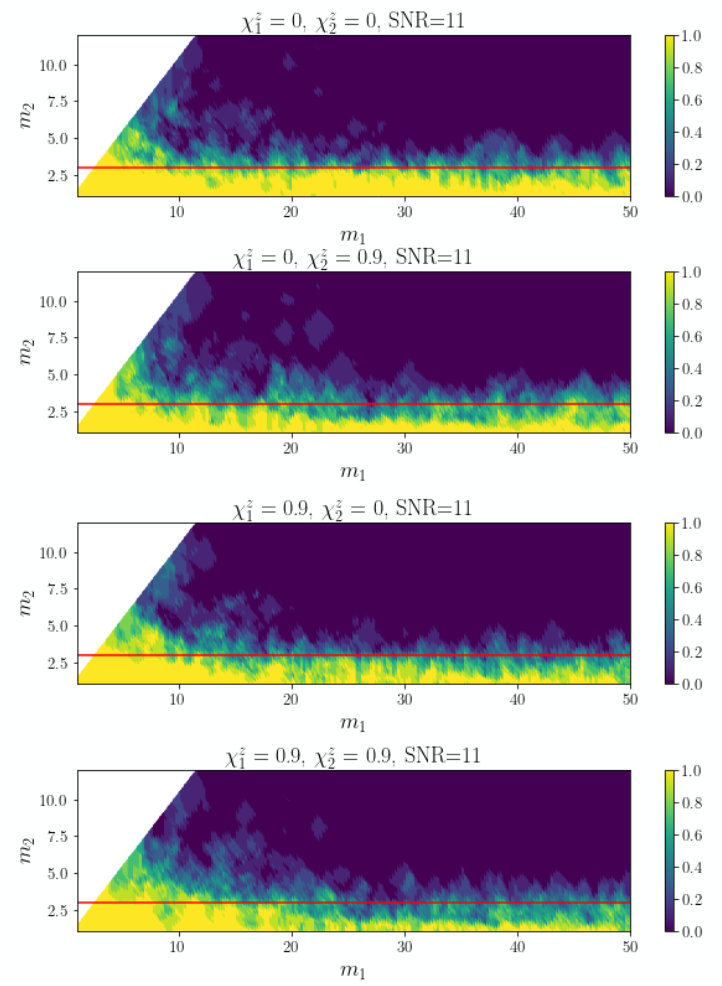
\includegraphics[width = 0.4\textwidth]{plot_fig4_chatt_spins.png}
  %   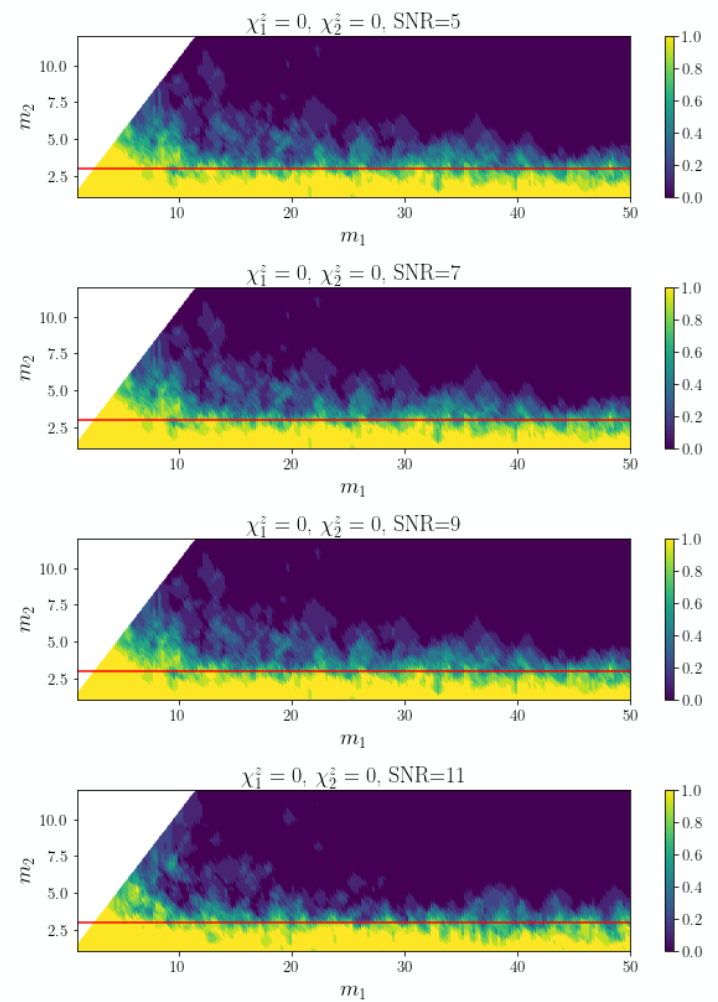
\includegraphics[width = 0.4\textwidth]{/Users/miquelmiravet/Projects/IPAM_LA/ML_group/IPAM2021_ML/algo/classy_KNN/PLOTS_KNN/NS_set/plots_miq/plot_fig4_chatt_snr.png}
    \caption{Probability of having a remnant as a function of the values of the masses. The different panels show the results for different spins. The solid red line depicts the threshold mass for $m_2$.}
    \label{fig:m1m2}
\end{figure}

\begin{figure}
	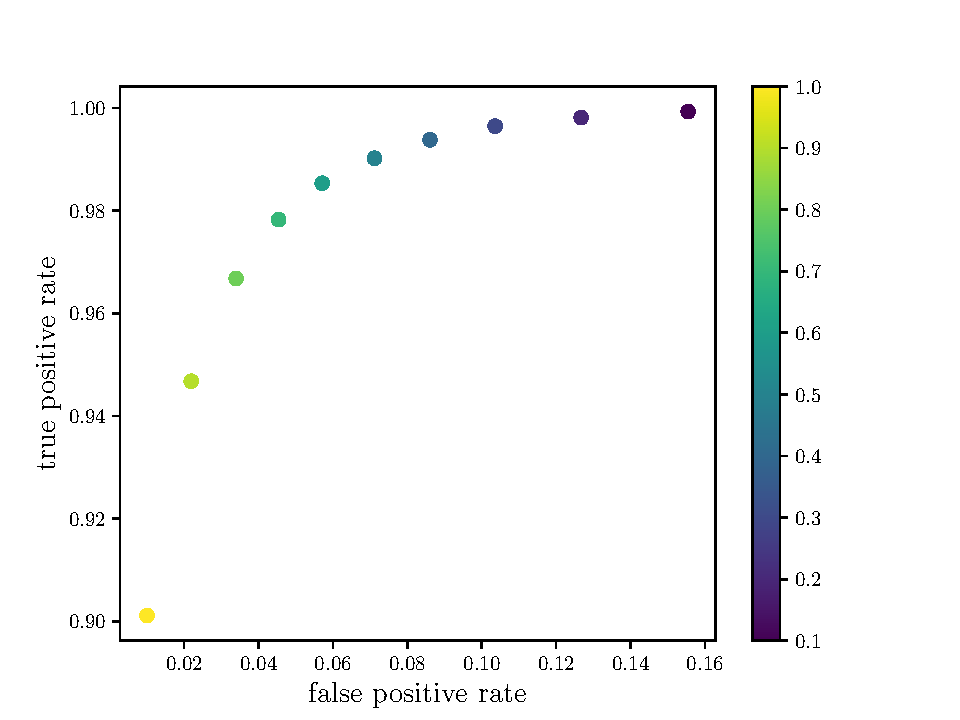
\includegraphics[width =0.4\textwidth]{ROCplot.pdf}
    \caption{Relation of the true and false positive rates as a function of the threshold applied to make the decision between having or not having a remnant. }
    \label{fig:roc}
\end{figure}

\mmt{In Fig.~\ref{fig:crossvalK} you can find how the mean score changes with the number of neighbors of the algorithm.  The confusion matrix appears in Fig.~\ref{fig:confmat}, the probability as a function of $m_1$ and $m_2$  is shown in Figs.~\ref{fig:m1m2}, and the true and false positive rates in terms of the threshold probability appear in Fig.~\ref{fig:roc}.}


 %plots and comments
\subsection{RF Results}

We apply crossvalidation in the number of trees and depth of the forests for the 23 EoS, fixing the information gain criteria to \texttt{entropy}. We also save the second best option for comparison, and save both forests for each EoS in order to compare the file size. As the goal is to provide a model that can run in a low latency pipeline the amount of memory it can take is limited, even more when there will be 23 different model for the EoS generalization.

In table \ref{tab:RFcross} we present a summary of best and second best hyperparameters found in the crossvalidation for each EoS, along the memory the model occupies and the difference in the score. As we can see, usually a forest with many trees has a second best option with far less that is lighter in memory and achieves a similar performance. The optimum maximum depth is always 15. Also the score achieved for every EoS is similar, and so we check that our accuracy is not NS model dependent.

\begin{table*}[h]
\centering
\begin{tabular}{@{}lcccccccc@{}}
\toprule
                                & \multicolumn{4}{c}{Best}                                & \multicolumn{4}{c}{Second best}                            \\ \midrule
\multicolumn{1}{|l|}{EOS}       & Trees & Depth & Size(MB)    & \multicolumn{1}{c|}{Score}      & Trees & Depth & Size(MB)    & \multicolumn{1}{c|}{$\Delta$score} \\ \midrule
\multicolumn{1}{|l|}{APR4\_BB}  & 300   & 15    & 94.7  & \multicolumn{1}{c|}{0.9683018}  & 50    & 15    & 15.7  & \multicolumn{1}{c|}{3.35e-5}       \\ \midrule
\multicolumn{1}{|l|}{BHF\_BBB2} & 80    & 15    & 24.4  & \multicolumn{1}{c|}{0.9685127}  & 300   & 15    & 91.6  & \multicolumn{1}{c|}{5.16e-5}       \\ \midrule
\multicolumn{1}{|l|}{H4}        & 80    & 15    & 29.6  & \multicolumn{1}{c|}{0.9618587}  & 300   & 15    & 111.4 & \multicolumn{1}{c|}{1.19e-4}       \\ \midrule
\multicolumn{1}{|l|}{HQC18}     & 300   & 15    & 93.7  & \multicolumn{1}{c|}{0.9673755}  & 100   & 15    & 31.3  & \multicolumn{1}{c|}{3.06e-4}       \\ \midrule
\multicolumn{1}{|l|}{KDE0V}     & 300   & 15    & 92.0  & \multicolumn{1}{c|}{0.9673295}  & 80    & 15    & 24.5  & \multicolumn{1}{c|}{2.06e-4}       \\ \midrule
\multicolumn{1}{|l|}{KDE0V1}    & 100   & 15    & 30.9  & \multicolumn{1}{c|}{0.96704954} & 80    & 15    & 24.5  & \multicolumn{1}{c|}{3.43e-5}       \\ \midrule
\multicolumn{1}{|l|}{MPA1}      & 80    & 15    & 27.2  & \multicolumn{1}{c|}{0.96601225} & 300   & 15    & 102.1 & \multicolumn{1}{c|}{8.19e-5}       \\ \midrule
\multicolumn{1}{|l|}{MS1\_PP}   & 300   & 15    & 113.5 & \multicolumn{1}{c|}{0.96563534} & 80    & 15    & 30.2  & \multicolumn{1}{c|}{1.15e-4}       \\ \midrule
\multicolumn{1}{|l|}{MS1B\_PP}  & 300   & 15    & 114.2 & \multicolumn{1}{c|}{0.96555340} & 100   & 15    & 38.0  & \multicolumn{1}{c|}{1.97e-4}       \\ \midrule
\multicolumn{1}{|l|}{RS}        & 300   & 15    & 103.8 & \multicolumn{1}{c|}{0.96447350} & 80    & 15    & 27.6  & \multicolumn{1}{c|}{2.36e-4}       \\ \midrule
\multicolumn{1}{|l|}{SK255}     & 300   & 15    & 105.8 & \multicolumn{1}{c|}{0.96472405} & 100   & 15    & 35.5  & \multicolumn{1}{c|}{3.69e-4}       \\ \midrule
\multicolumn{1}{|l|}{SK272}     & 300   & 15    & 109.0 & \multicolumn{1}{c|}{0.96401816} & 100   & 15    & 36.4  & \multicolumn{1}{c|}{1.99e-4}       \\ \midrule
\multicolumn{1}{|l|}{SKI2}      & 50    & 15    & 18.8  & \multicolumn{1}{c|}{0.96242338} & 300   & 15    & 112.8 & \multicolumn{1}{c|}{8.37e-5}       \\ \midrule
\multicolumn{1}{|l|}{SKI3}      & 50    & 15    & 19.0  & \multicolumn{1}{c|}{0.96174537} & 100   & 15    & 38.1  & \multicolumn{1}{c|}{6.62e-5}       \\ \midrule
\multicolumn{1}{|l|}{SKI4}      & 300   & 15    & 100.6 & \multicolumn{1}{c|}{0.96598969} & 30    & 15    & 9.8   & \multicolumn{1}{c|}{8.37e-5}       \\ \midrule
\multicolumn{1}{|l|}{SKI5}      & 100   & 15    & 38.2  & \multicolumn{1}{c|}{0.96343381} & 80    & 15    & 30.4  & \multicolumn{1}{c|}{1.16e-4}       \\ \midrule
\multicolumn{1}{|l|}{SKI6}      & 300   & 15    & 101.7 & \multicolumn{1}{c|}{0.96586928} & 30    & 15    & 10.0  & \multicolumn{1}{c|}{2.17e-4}       \\ \midrule
\multicolumn{1}{|l|}{SKMP}      & 300   & 15    & 100.2 & \multicolumn{1}{c|}{0.96544567} & 80    & 15    & 26.9  & \multicolumn{1}{c|}{1.69e-4}       \\ \midrule
\multicolumn{1}{|l|}{SKOP}      & 100   & 15    & 32.3  & \multicolumn{1}{c|}{0.96610459} & 300   & 15    & 96.2  & \multicolumn{1}{c|}{6.85e-5}       \\ \midrule
\multicolumn{1}{|l|}{SLy}       & 80    & 15    & 25.3  & \multicolumn{1}{c|}{0.96728884} & 300   & 15    & 95.2  & \multicolumn{1}{c|}{8.49e-5}       \\ \midrule
\multicolumn{1}{|l|}{SLY2}      & 100   & 15    & 31.8  & \multicolumn{1}{c|}{0.96745868} & 80    & 15    & 25.4  & \multicolumn{1}{c|}{2.38e-4}       \\ \midrule
\multicolumn{1}{|l|}{SLY9}      & 300   & 15    & 101.6 & \multicolumn{1}{c|}{0.96605993} & 100   & 15    & 34.1  & \multicolumn{1}{c|}{1.51e-4}       \\ \midrule
SLY230A                         & 300   & 15    & 95.5  & 0.96714915                      & 100   & 15    & 31.9  & 2.53e-4                            \\ \bottomrule
\end{tabular}
\caption{Comparison of the best and second best RF models obtained during crossvalidation for all EoS. We show the file size in MB of the forest, and the difference in score between the two options.}
\label{tab:RFcross}
\end{table*}

To simplify the model and according to the results of crossvalidation, we train the final forests for all EoS with 50 trees and 15 maximum depth. In figure \ref{fig:RF_roc} we show the ROC curves for all models to give an idea of the performance. Notice that HasREM performs better than HasNS. The ourperformance of HasREM against HasNS in RF is even more noticeable in the histograms in figures \ref{fig:RF_hist_BHFBBB2}, \ref{fig:RF_hist_SLY} and \ref{fig:RF_hist_MS1PP} for the highlighted EoS, where the bars of asigned probabilities do not intersect each other and therefore there exists a threshold value for perfect classification in the testing dataset.

\begin{figure}
\centering
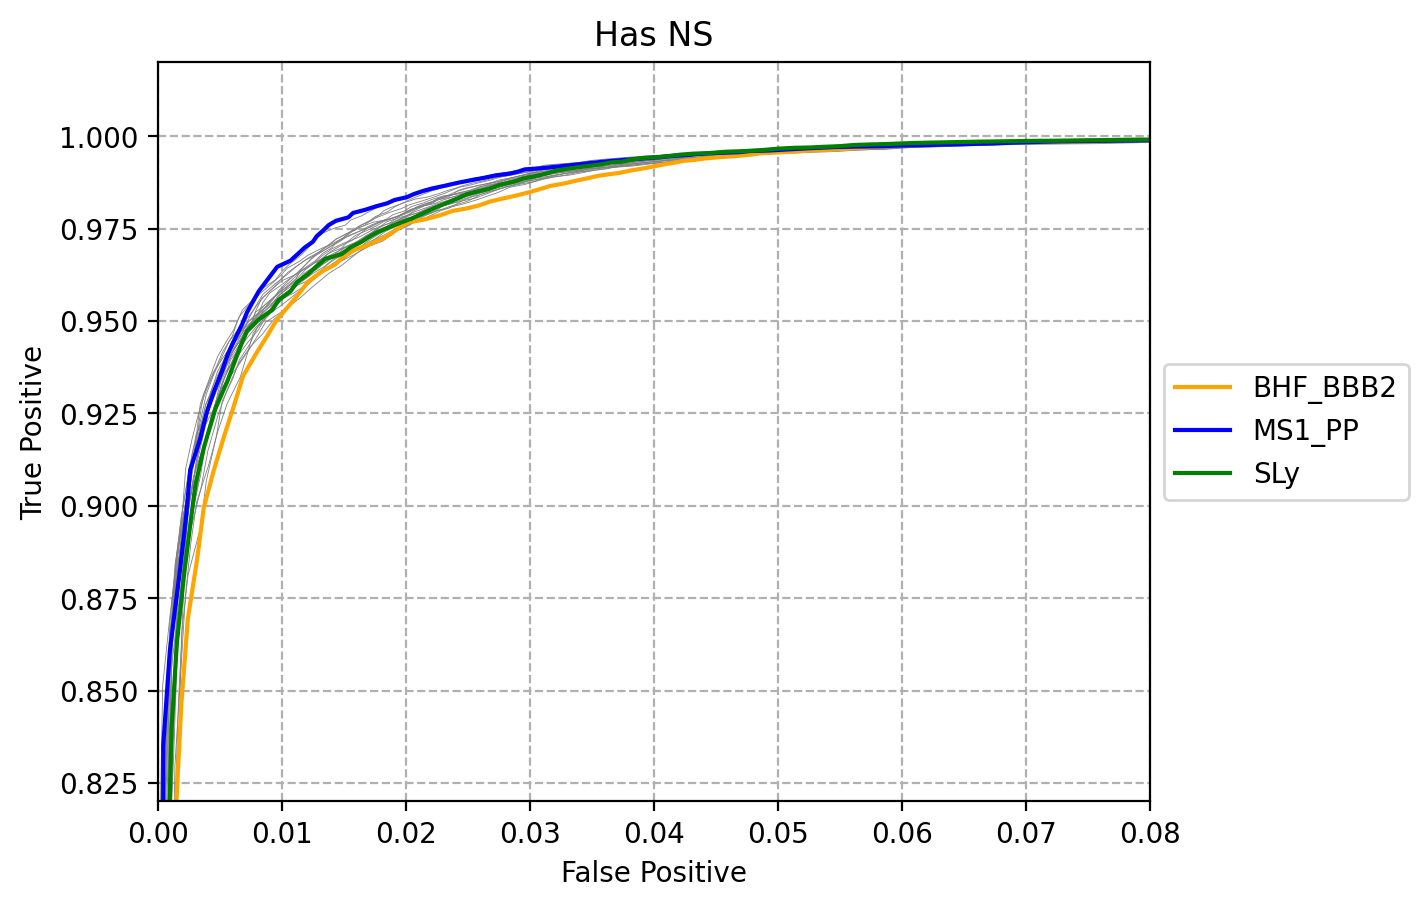
\includegraphics[width=0.45\textwidth]{/figs/HasNS_roc}
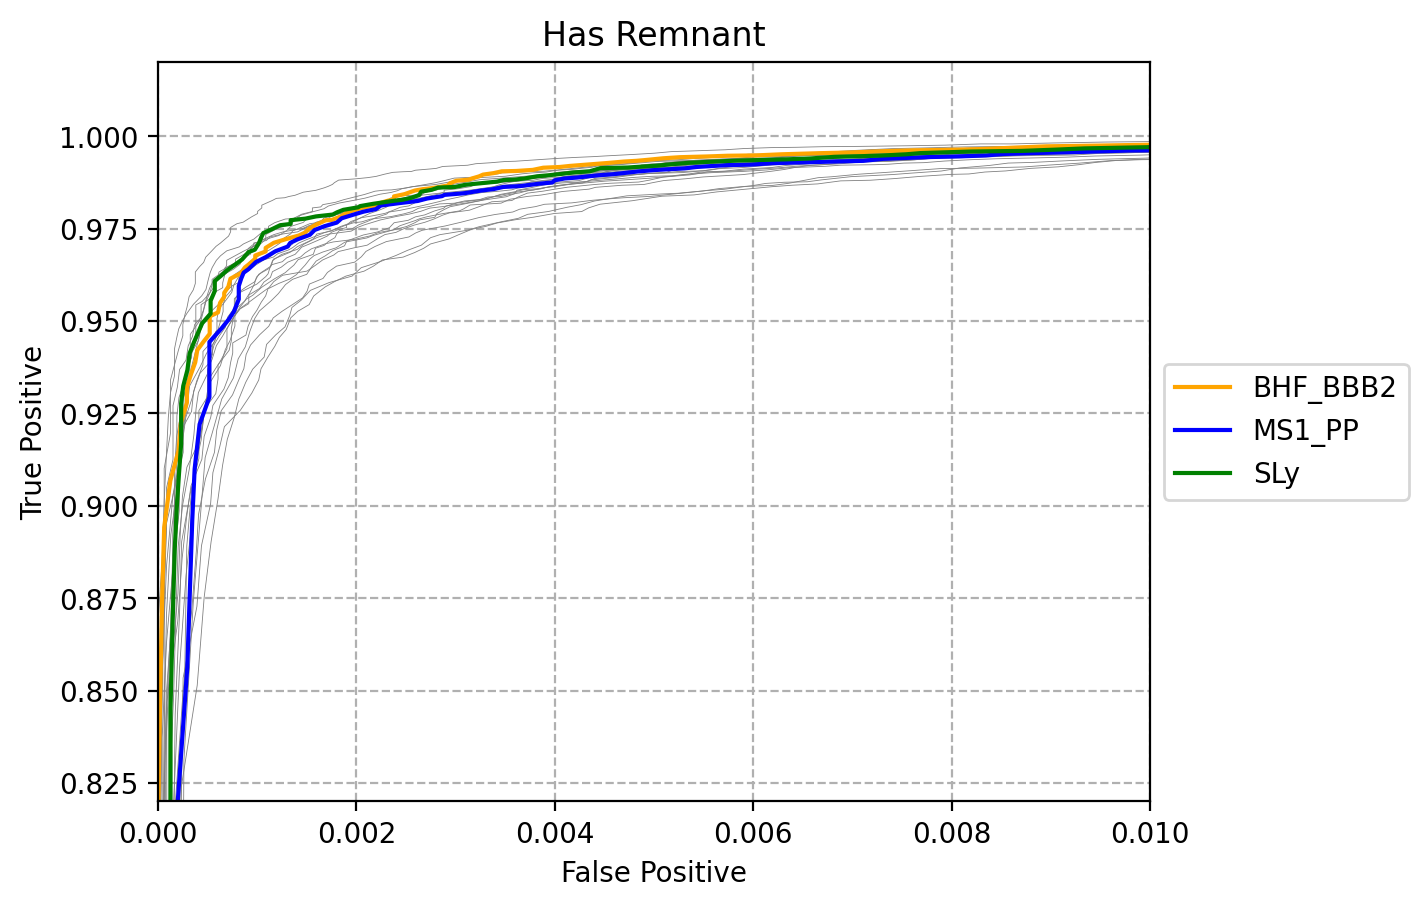
\includegraphics[width=0.45\textwidth]{/figs/HasREM_roc}
\caption{\label{fig:RF_roc} ROC curves}
\end{figure}

\begin{figure}
\centering
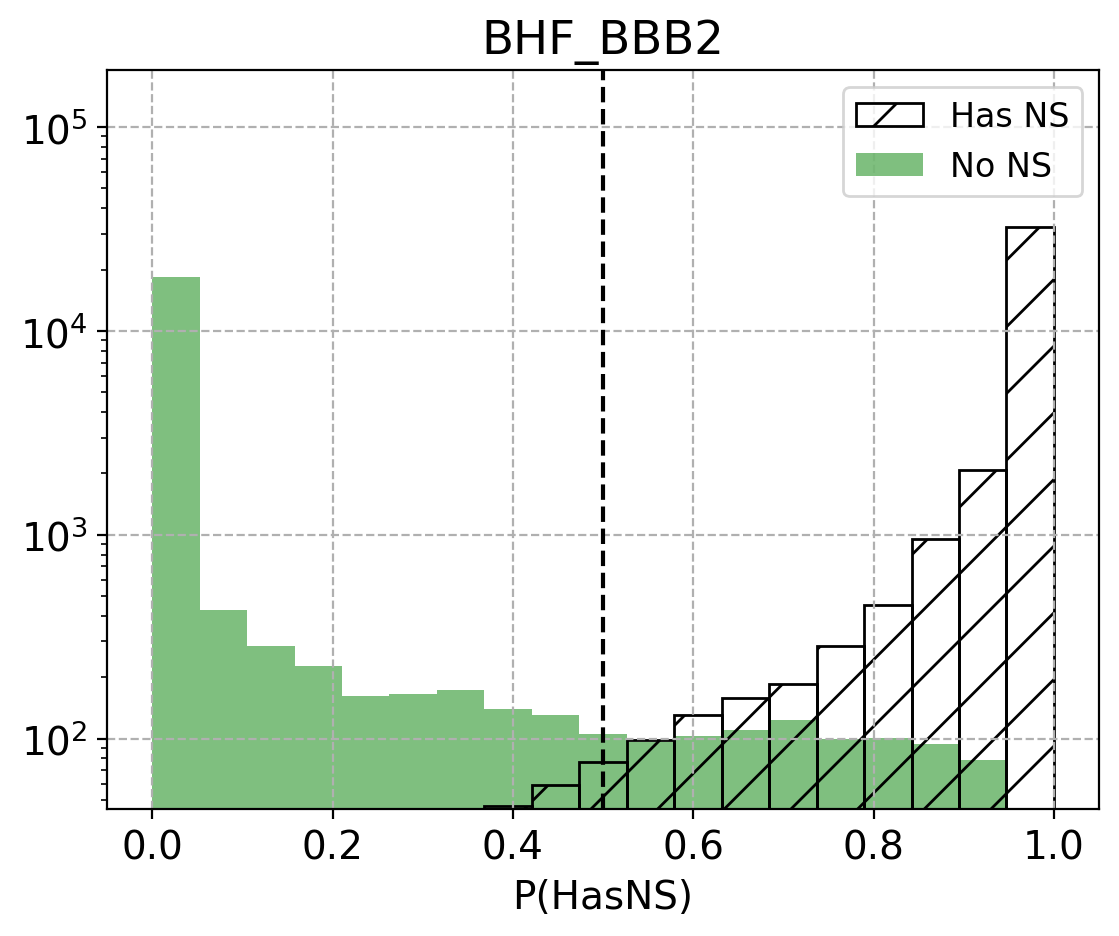
\includegraphics[width=0.45\textwidth]{/figs/BHF_BBB2_NShist}
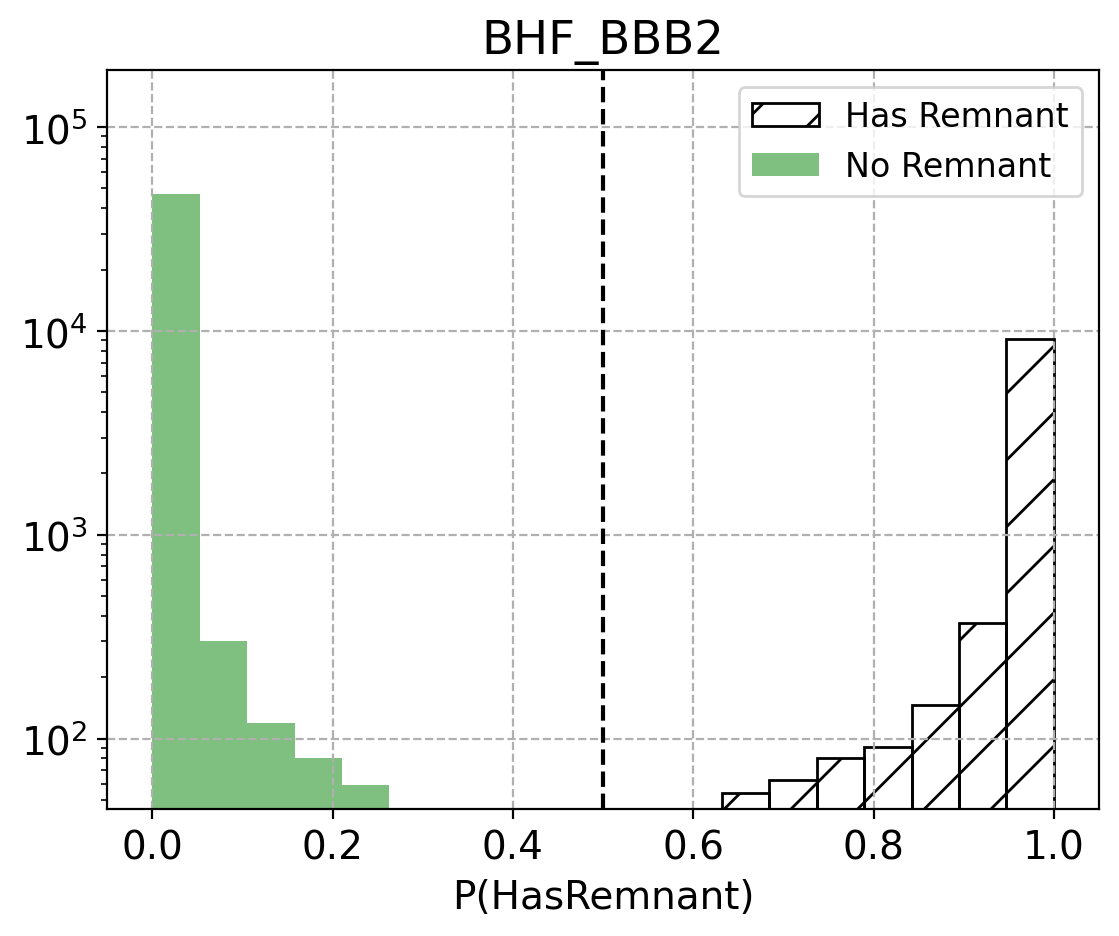
\includegraphics[width=0.45\textwidth]{/figs/BHF_BBB2_REMhist}
\caption{\label{fig:RF_hist_BHFBBB2} Histograms BHF BBB2}
\end{figure}

\begin{figure}
\centering
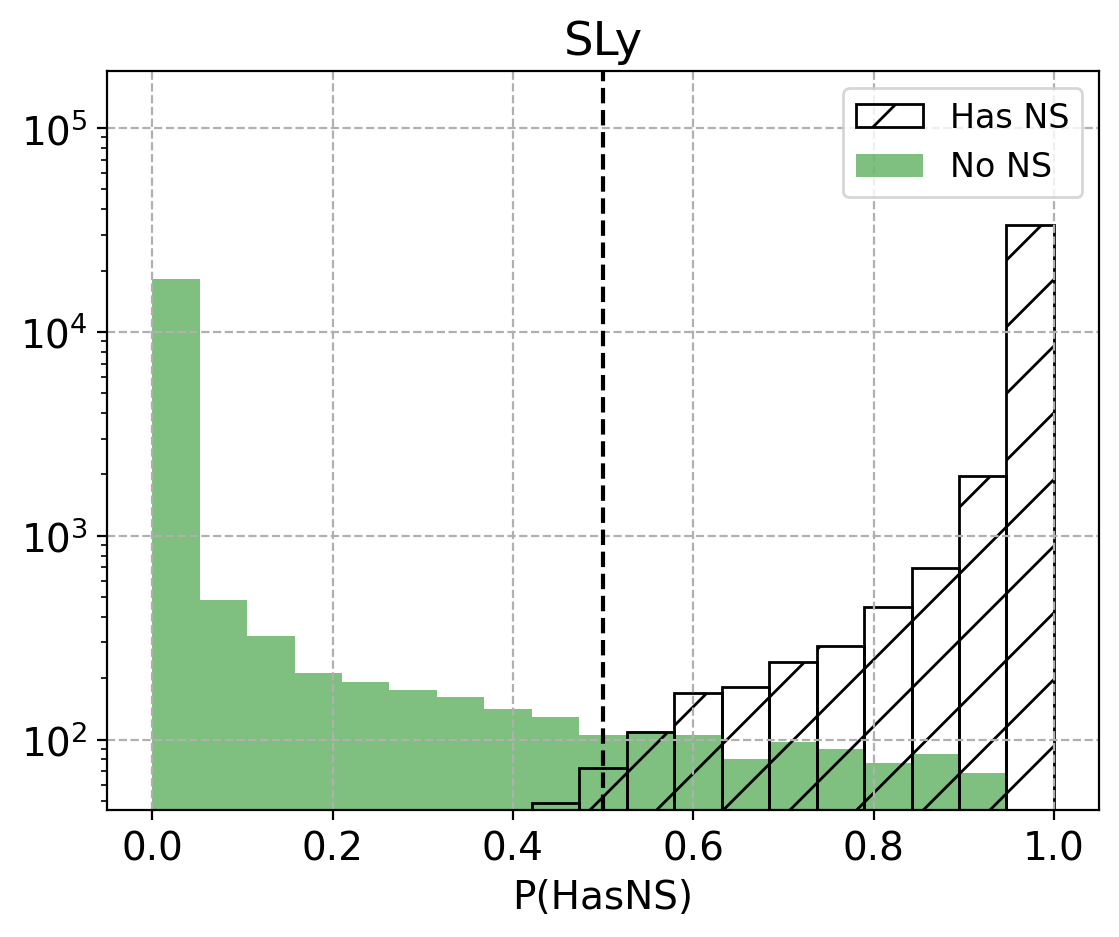
\includegraphics[width=0.45\textwidth]{/figs/SLy_NShist}
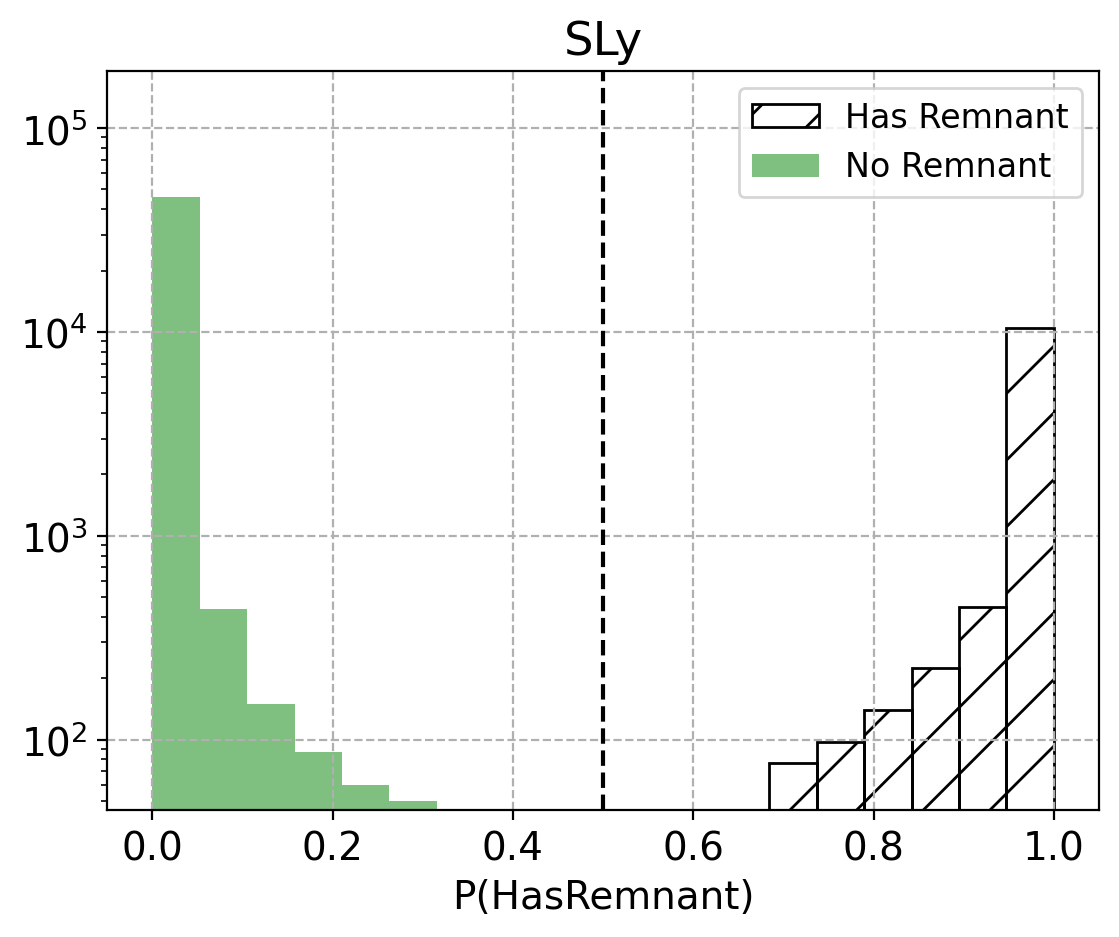
\includegraphics[width=0.45\textwidth]{/figs/SLy_REMhist}
\caption{\label{fig:RF_hist_SLY} Histograms SLy}
\end{figure}

\begin{figure}
\centering
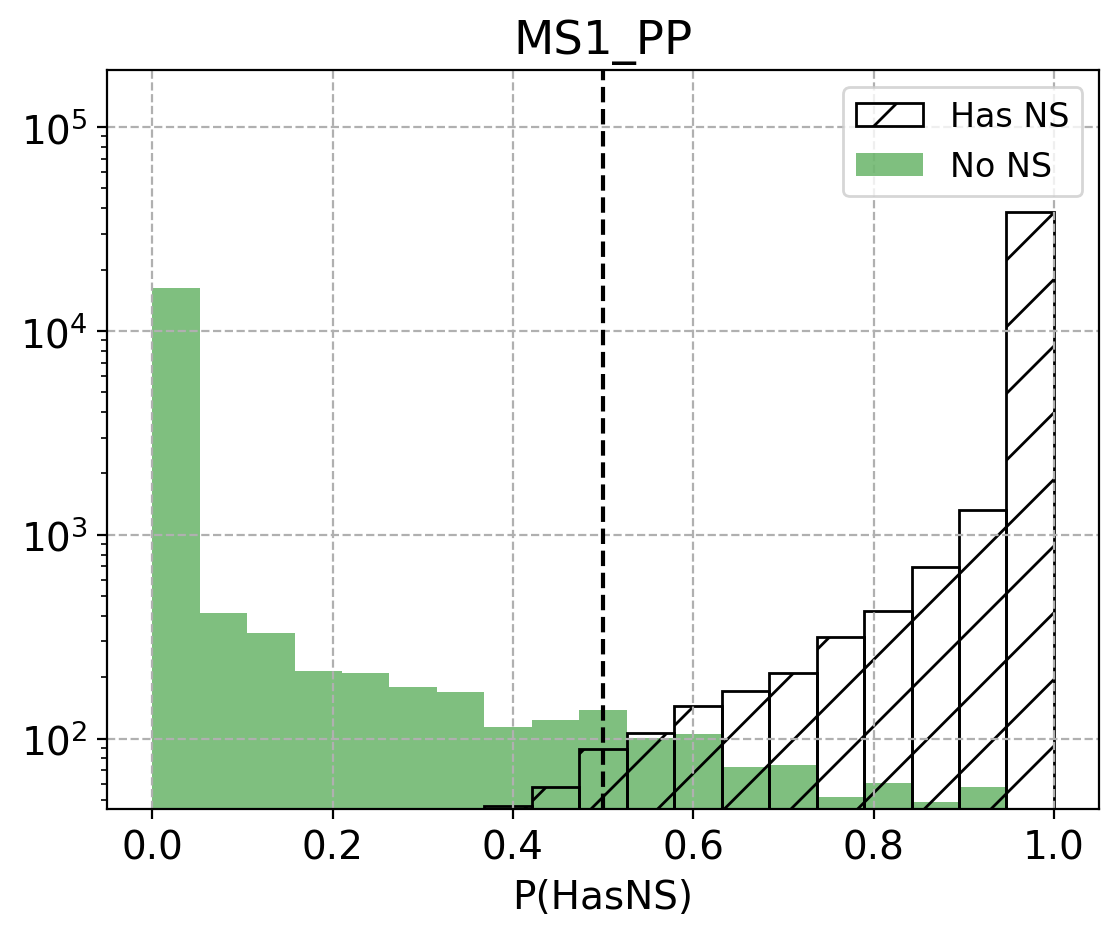
\includegraphics[width=0.45\textwidth]{/figs/MS1_PP_NShist}
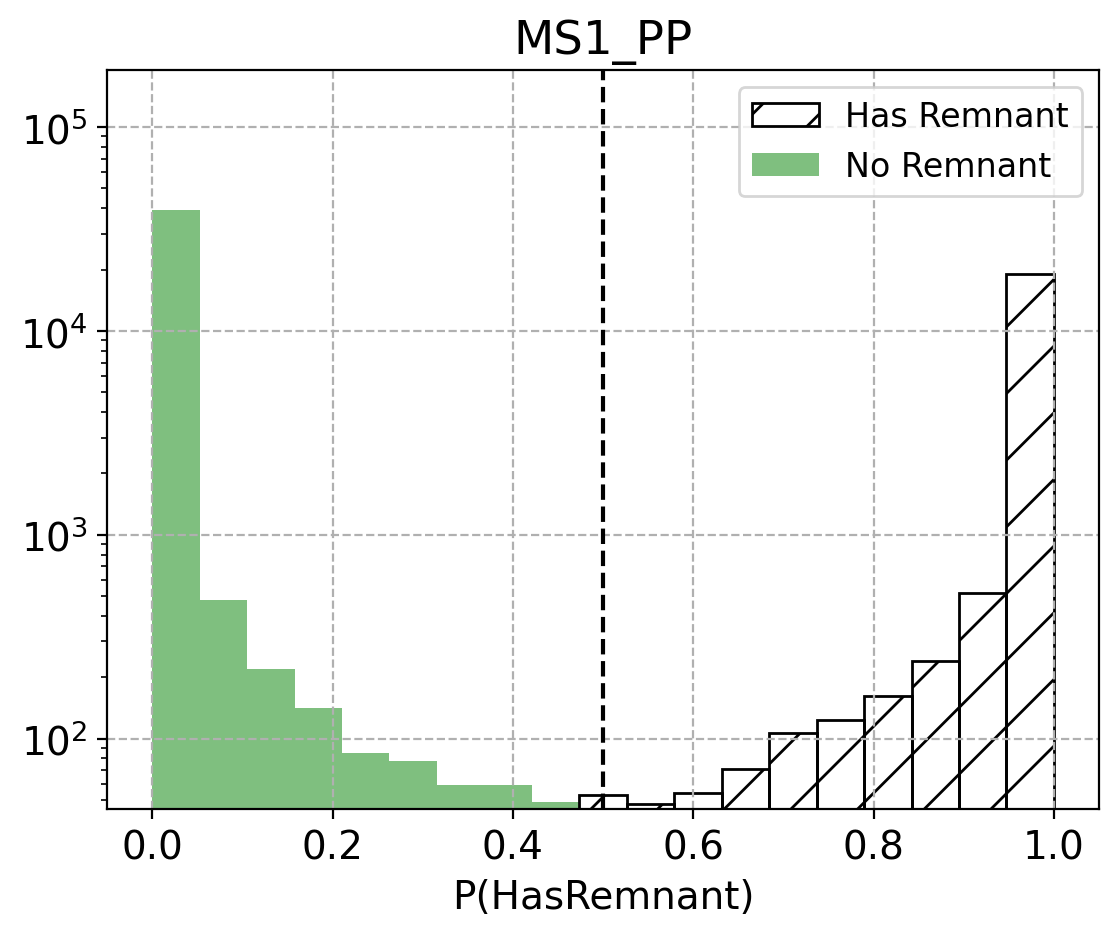
\includegraphics[width=0.45\textwidth]{/figs/MS1_PP_REMhist}
\caption{\label{fig:RF_hist_MS1PP} Histograms MS1 PP}
\end{figure}


 %plots and comments
\subsection{Algorithm comparison}
\section{Results\label{results}}
In this section we show the results for our methodology. First we illustrate the good performance of our classifiers, both \ac{RF} and \ac{KNN}. Then we can use them to construct Bayesian probabilities according to their output and finally evaluate new events, synthetic and real.

\subsection{Performance of the algorithms}
We measure the performance of our algorithms by the true positive and false positive rates, drawn as \textit{Receiver Operating Characteristic} (ROC) curves. They show the variation of the true-positive rate with the false-positive rate given a certain threshold for the probability. The better the classifier, the steeper is the curve achiving a greater number of true positives with very few false classifications.

The curves for \ac{KNN} are in figure \ref{fig:rocO2_KNN}. The results are consistent among all EoSs and represent a good classifier, with slitghly better results in the performance of \hasrem. The curves for \ac{RF} are in figure \ref{fig:rocO2_RF}. The results are equally good and consistent, showing that both classifiers perform similarly on the testing dataset.

\todo{UNIFY AXIS AND SIZE OF FIGURES}

\begin{figure}[h]
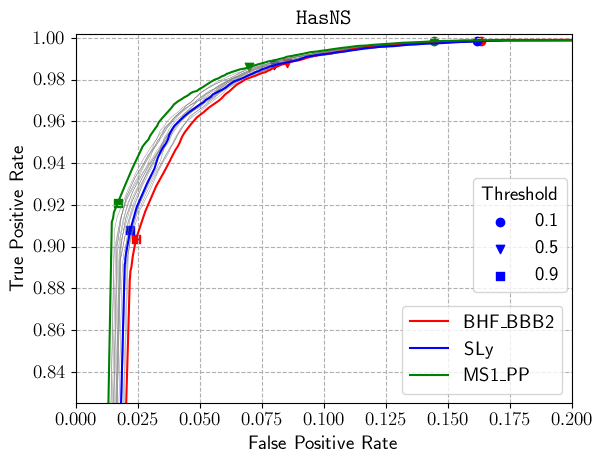
\includegraphics{roc_testing_KNN_NS}
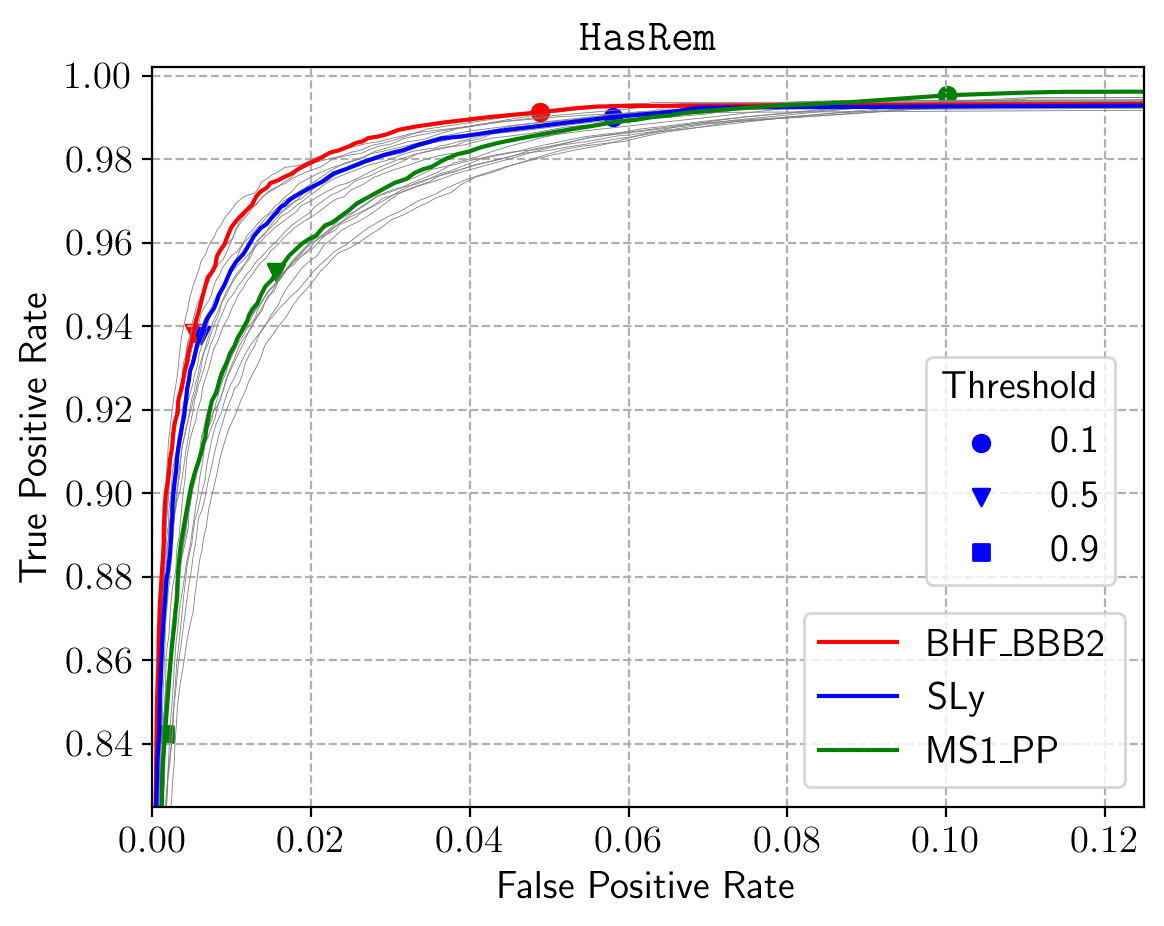
\includegraphics{roc_testing_KNN_REM}
\caption{\label{fig:rocO2_KNN}ROC curves for the testing dataset for \ac{KNN} classfier. All 23 EoS shown in grey, in color the EoSs with minimum and maximum mass, along commonly used SLy.}
\end{figure}

\begin{figure}[h]
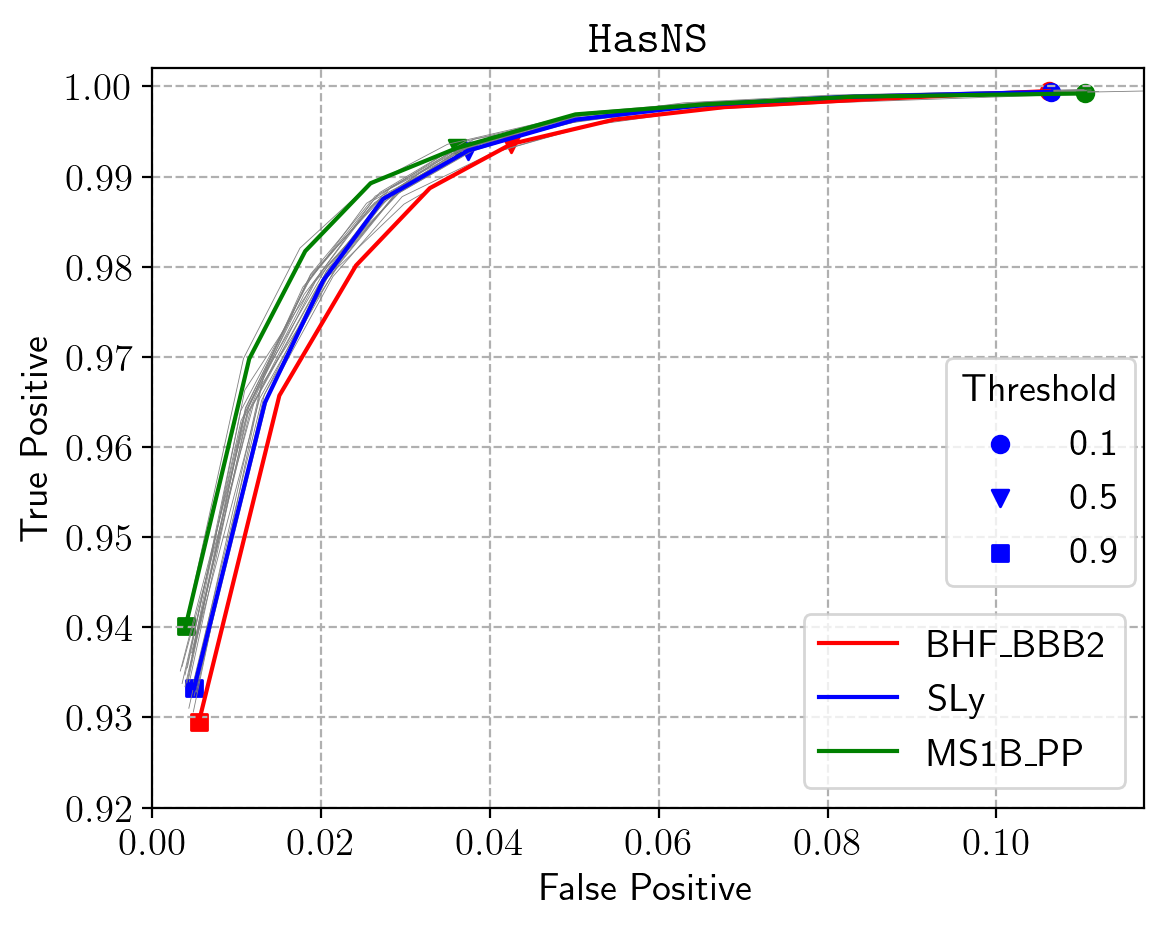
\includegraphics{ROC_O2testing_NS_RF}
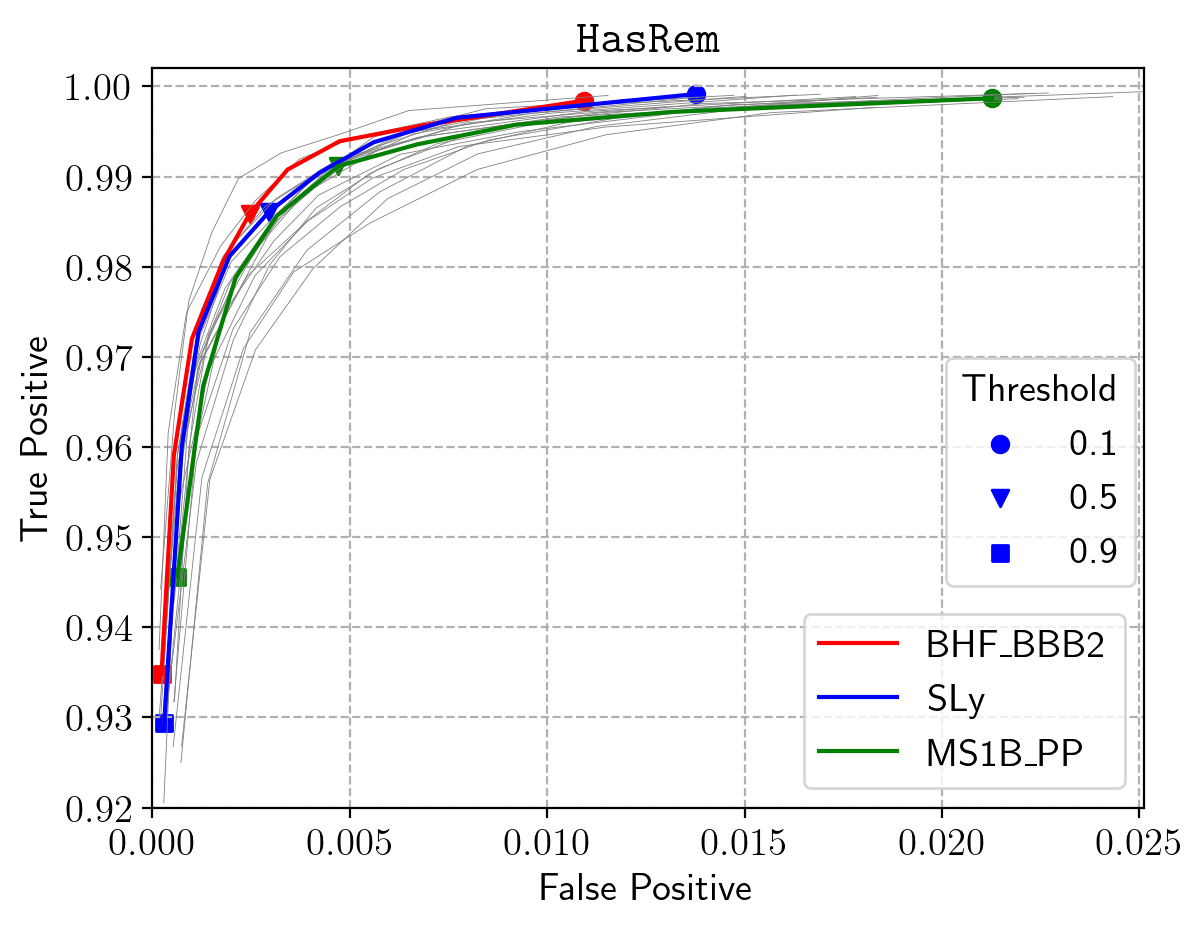
\includegraphics{ROC_O2testing_REM_RF}
\caption{\label{fig:rocO2_RF}ROC curves for the testing dataset for \ac{RF} classfier. All 23 EoS shown in grey, in color the EoSs with minimum and maximum mass, along commonly used SLy.}
\end{figure}



\subsection{Computation of the probabilities}
\todo{write the subsection}
Now that we have seen the performance, we compute the bayesian probs according to section whatever

plots fits (probability plot) (done I think, Miquel)
And with that we have probability tables

\subsection{Performance on new events}
We use the tables constructed \todo{write}
Table probs O3 detections (I think computed, just make sure it is good) \todo{introduce properly and put clean tables (they are below)}

We use the marginalized Bayesian probabilities obtained with both algorithms to classify the events in MDC11 \todo{explain? or was it explained before?}. We compute the ROC curves according the ground truth of the injected events. We separate the ROC curves for the different pipelines involved in the dataset. Notice that the performance for all of them is good even if the training and computing of probabilities was performed using GstLAL exclusively. Figure \ref{fig:rocMDC_KNN} depicts the curves for KNN. It performs very well for \hasns achieving a true positive rate very close to unity with a very small false positive rate. We observe that spiir pipeline deviates from the good behaviour. For \hasrem the overall performance is slightly worse, getting higher false positive rate, but in turn all pipelines behave equally good. In figure \ref{fig:rocMDC_RF} we showcase the results for \ac{RF}. As with \ac{KNN} the results are very good, with steep ROC curves. For \hasns spiir pipeline deviates less from the rest, getting higher positive rates for the same false positives than with \ac{KNN}. In the case of \hasrem the curves of the different pipelines behave a bit more differently from each other.

\begin{figure}[h]
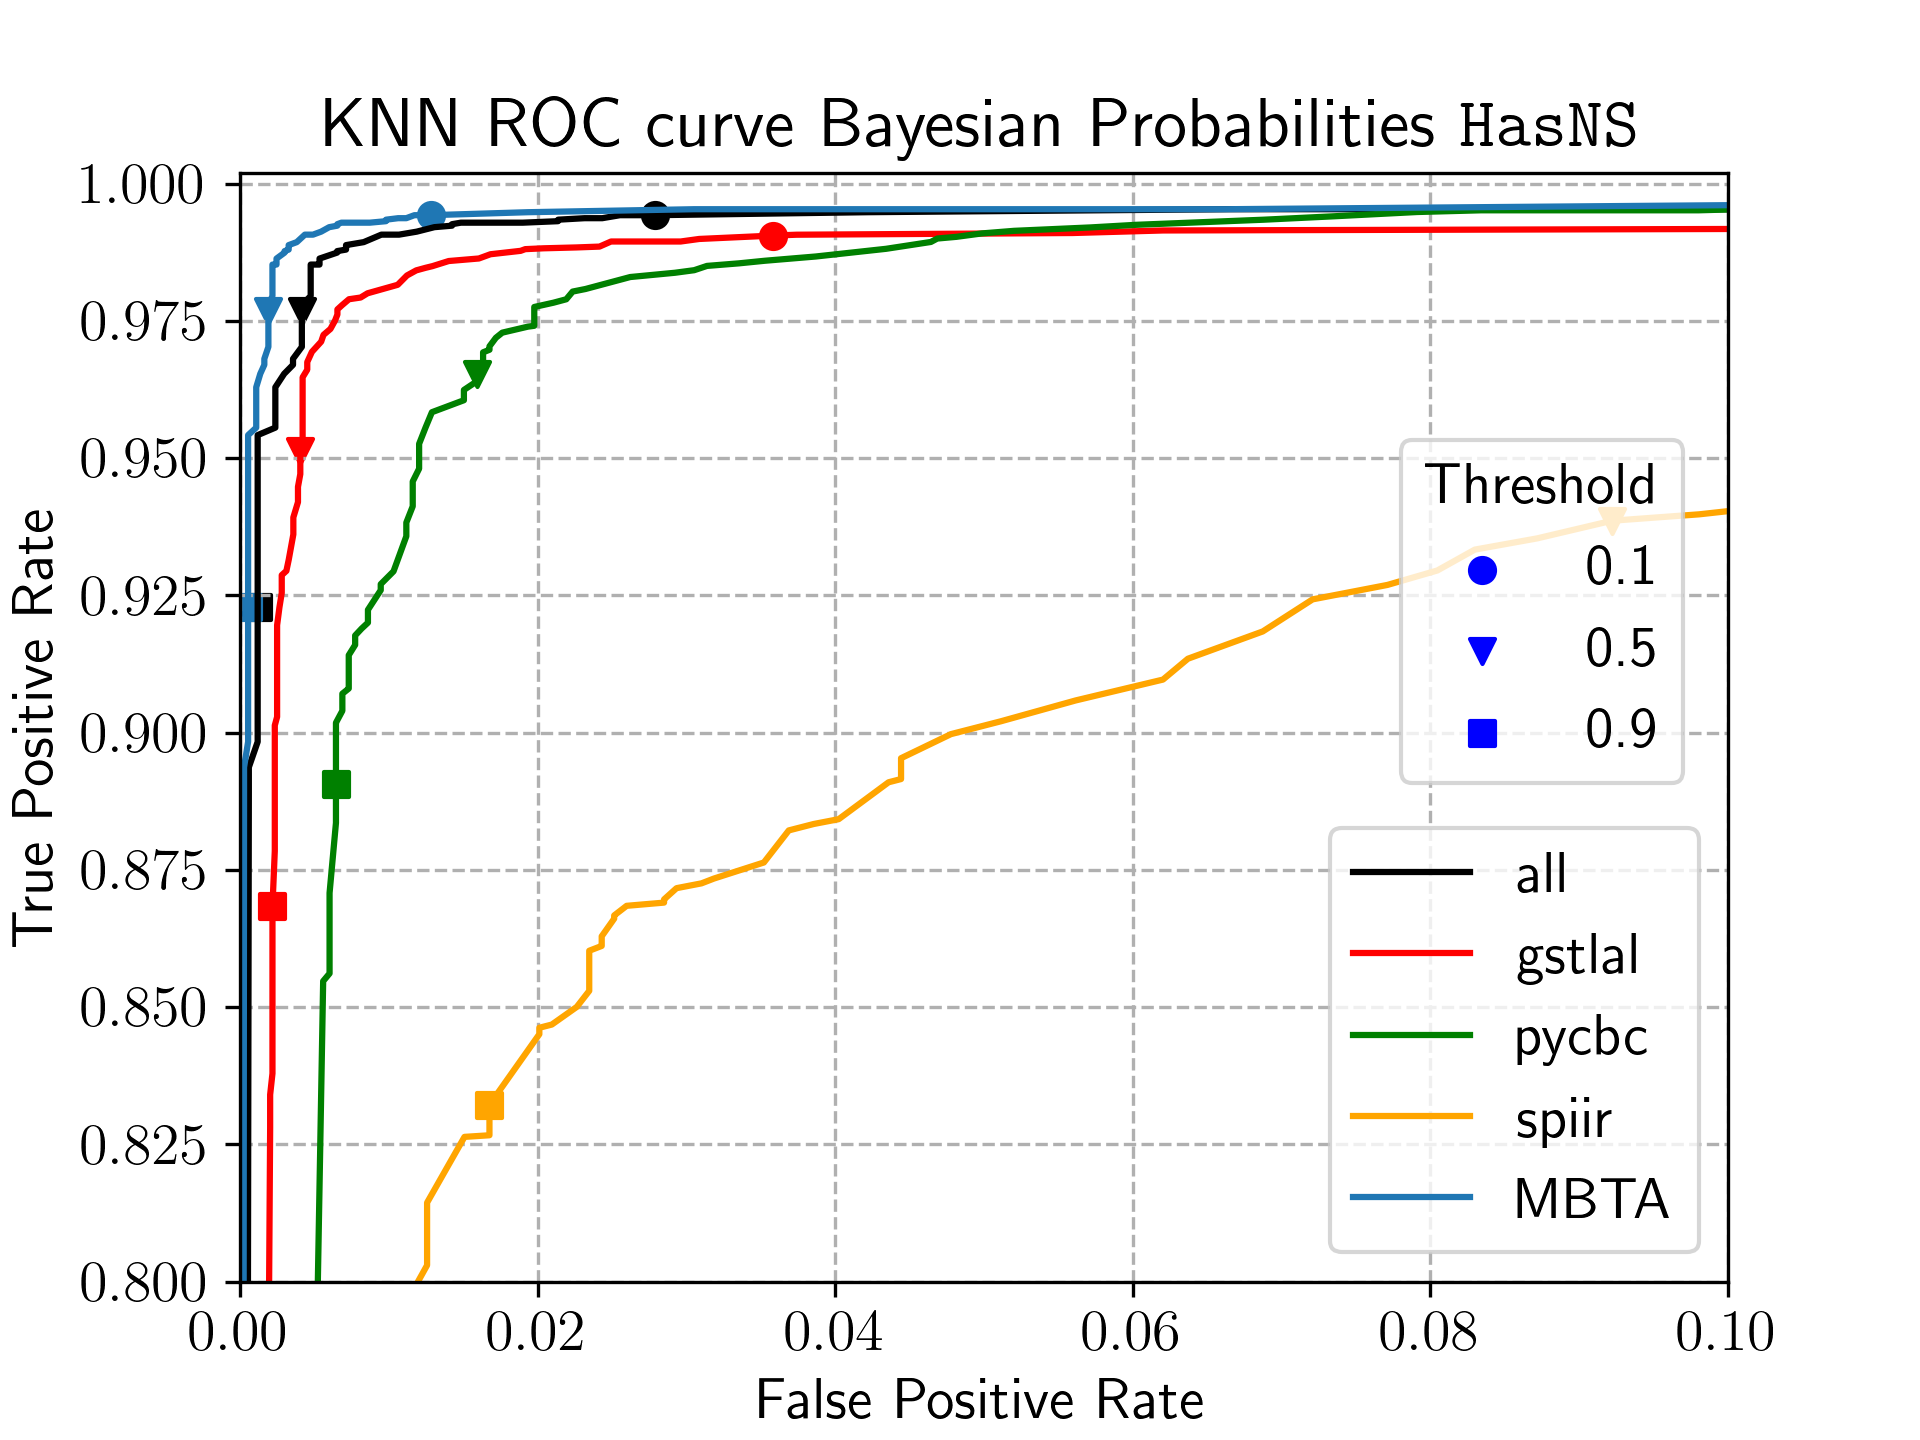
\includegraphics{KNN_bayesian_NS}
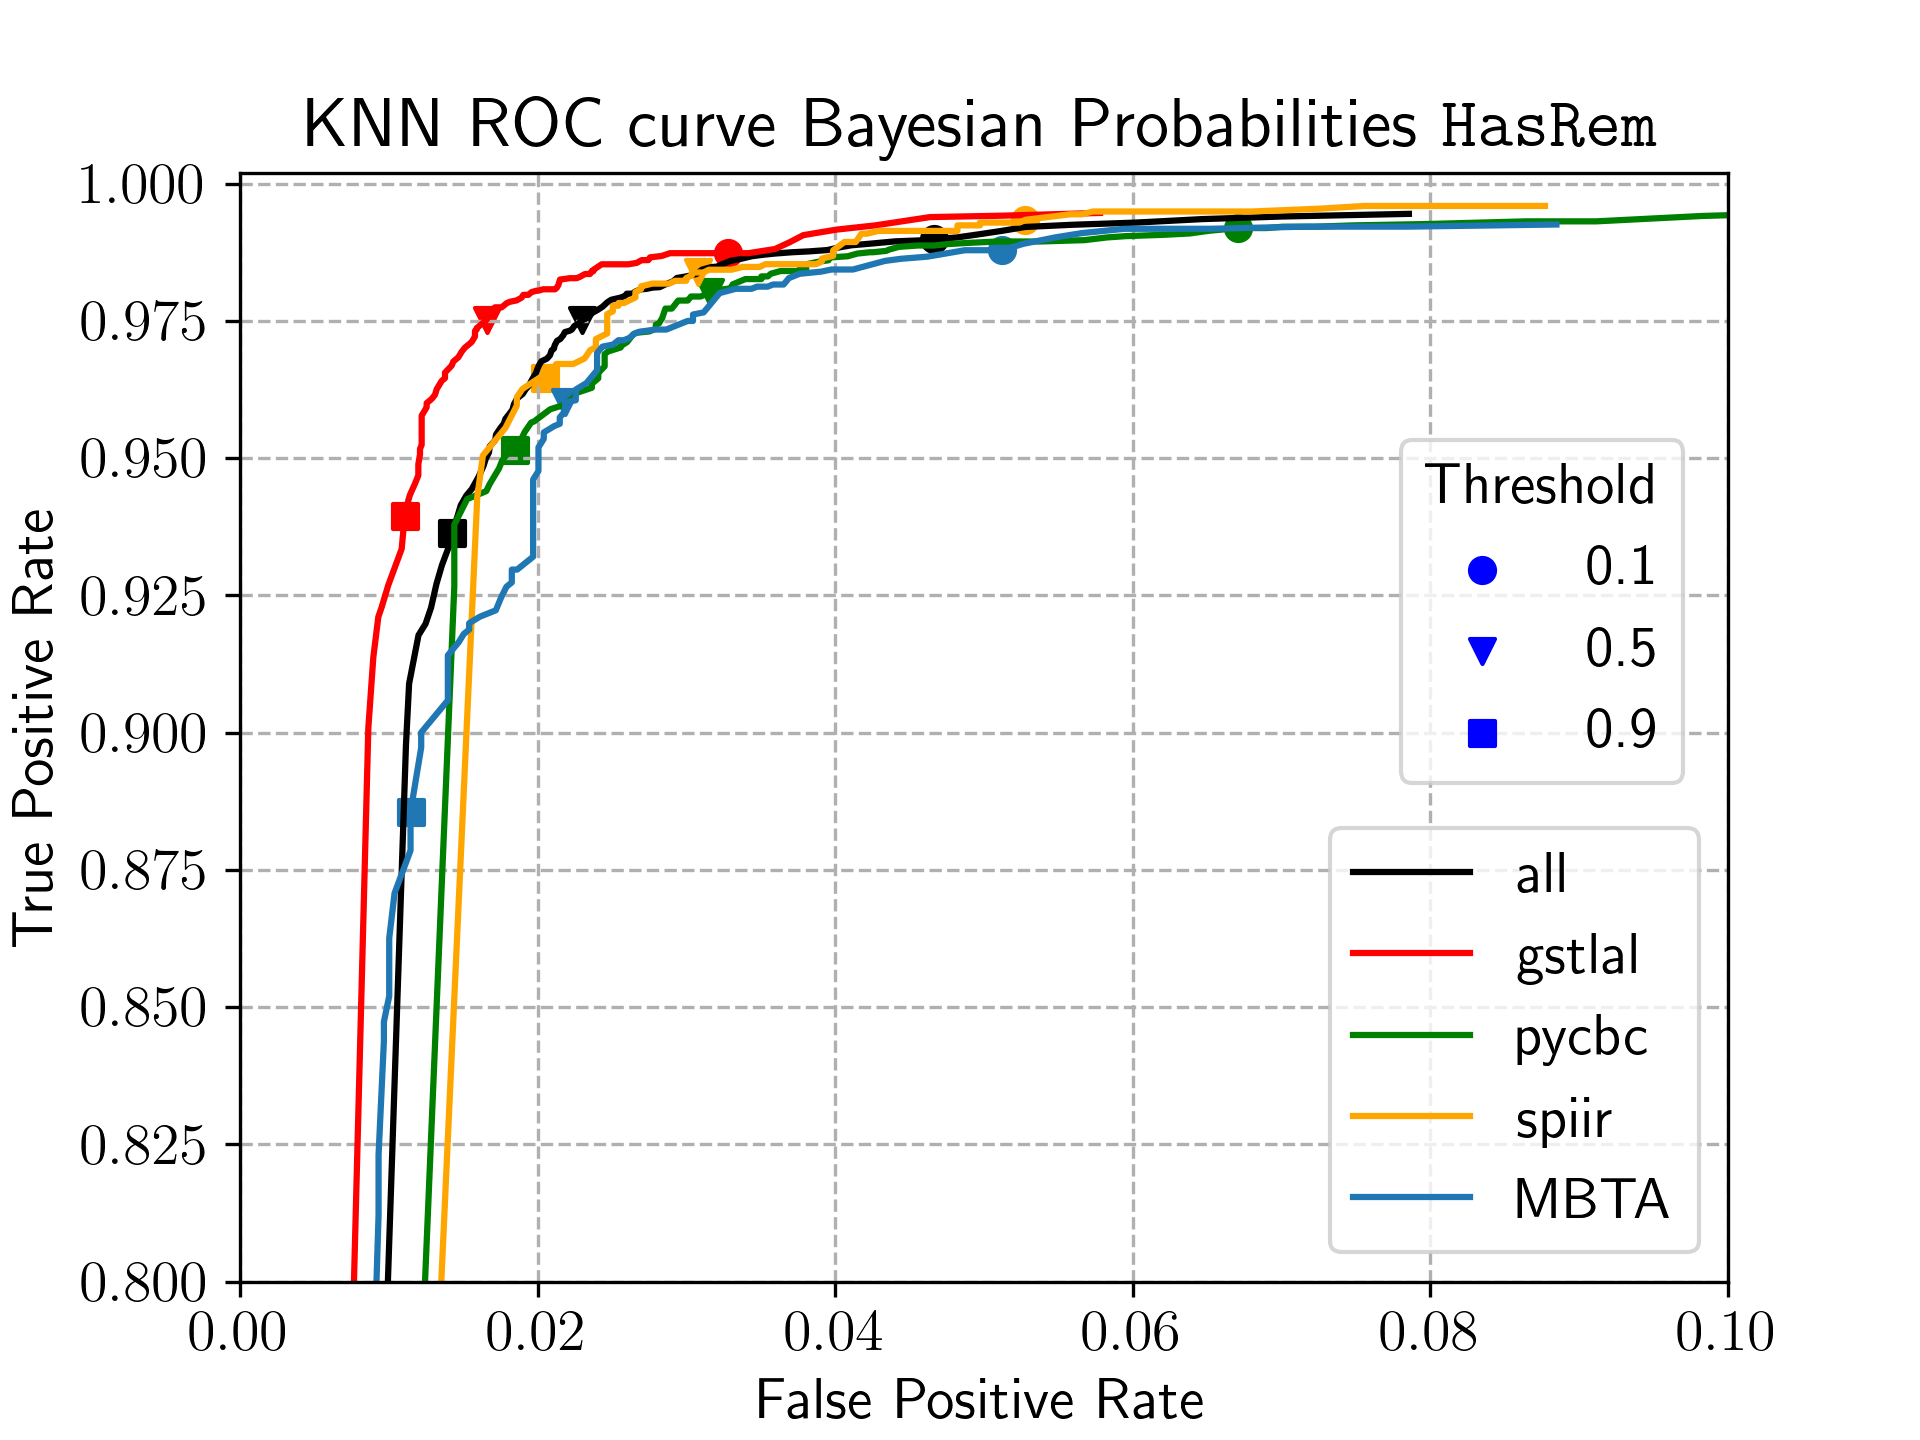
\includegraphics{KNN_bayesian_REM}
\caption{\label{fig:rocMDC_KNN}ROC curves of Bayesian probability marginalized for the 23 EoSs for MDC11 dataset using \ac{KNN} classifier.}
\end{figure}

\begin{figure}[h]
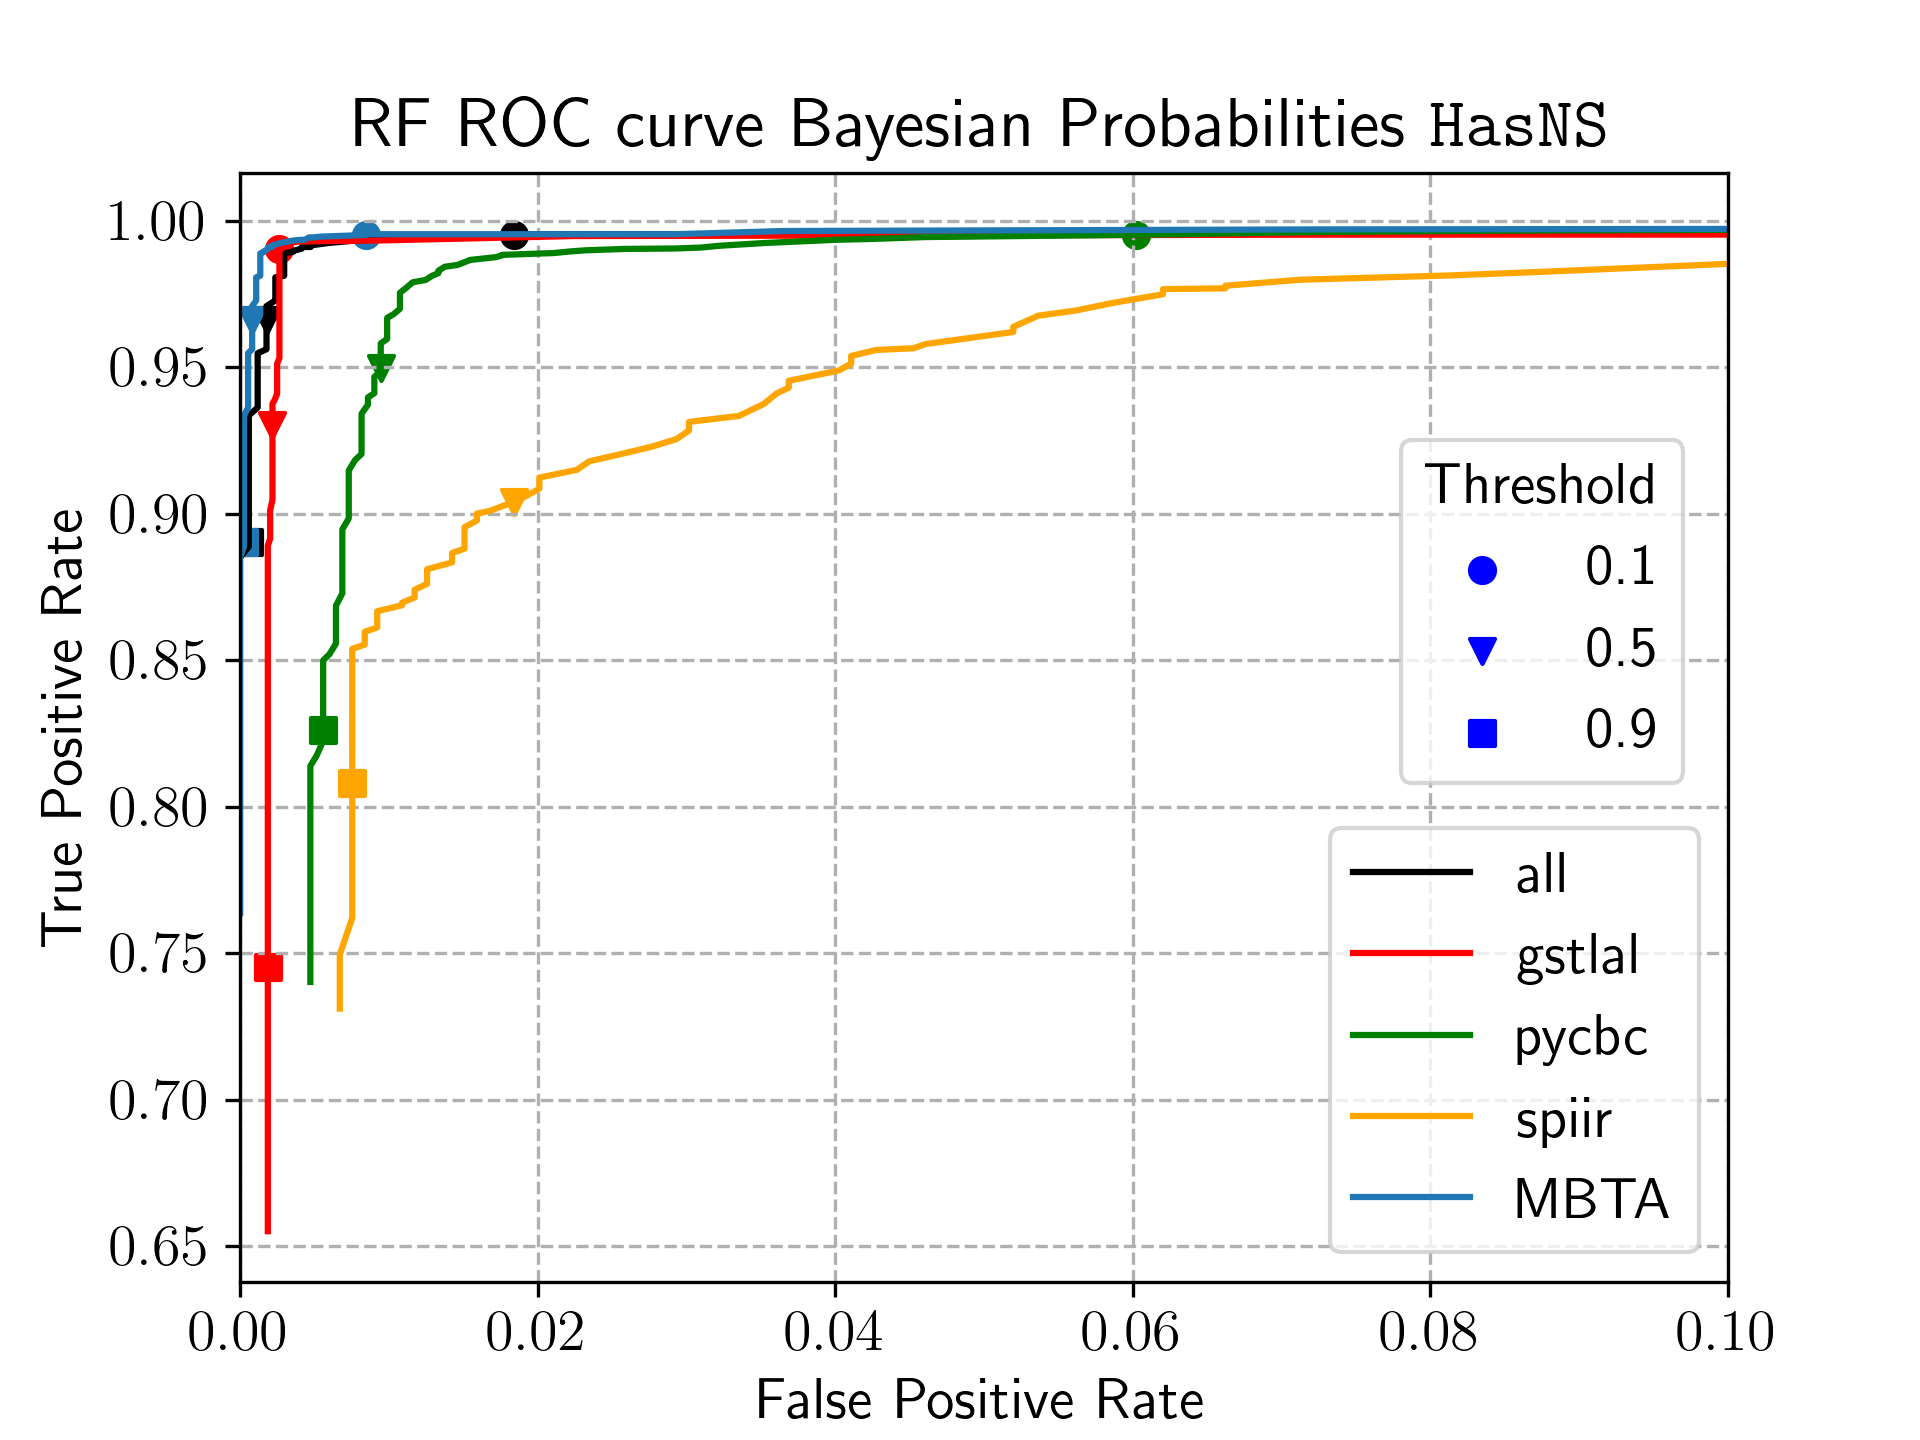
\includegraphics{RF_bayesian_NS}
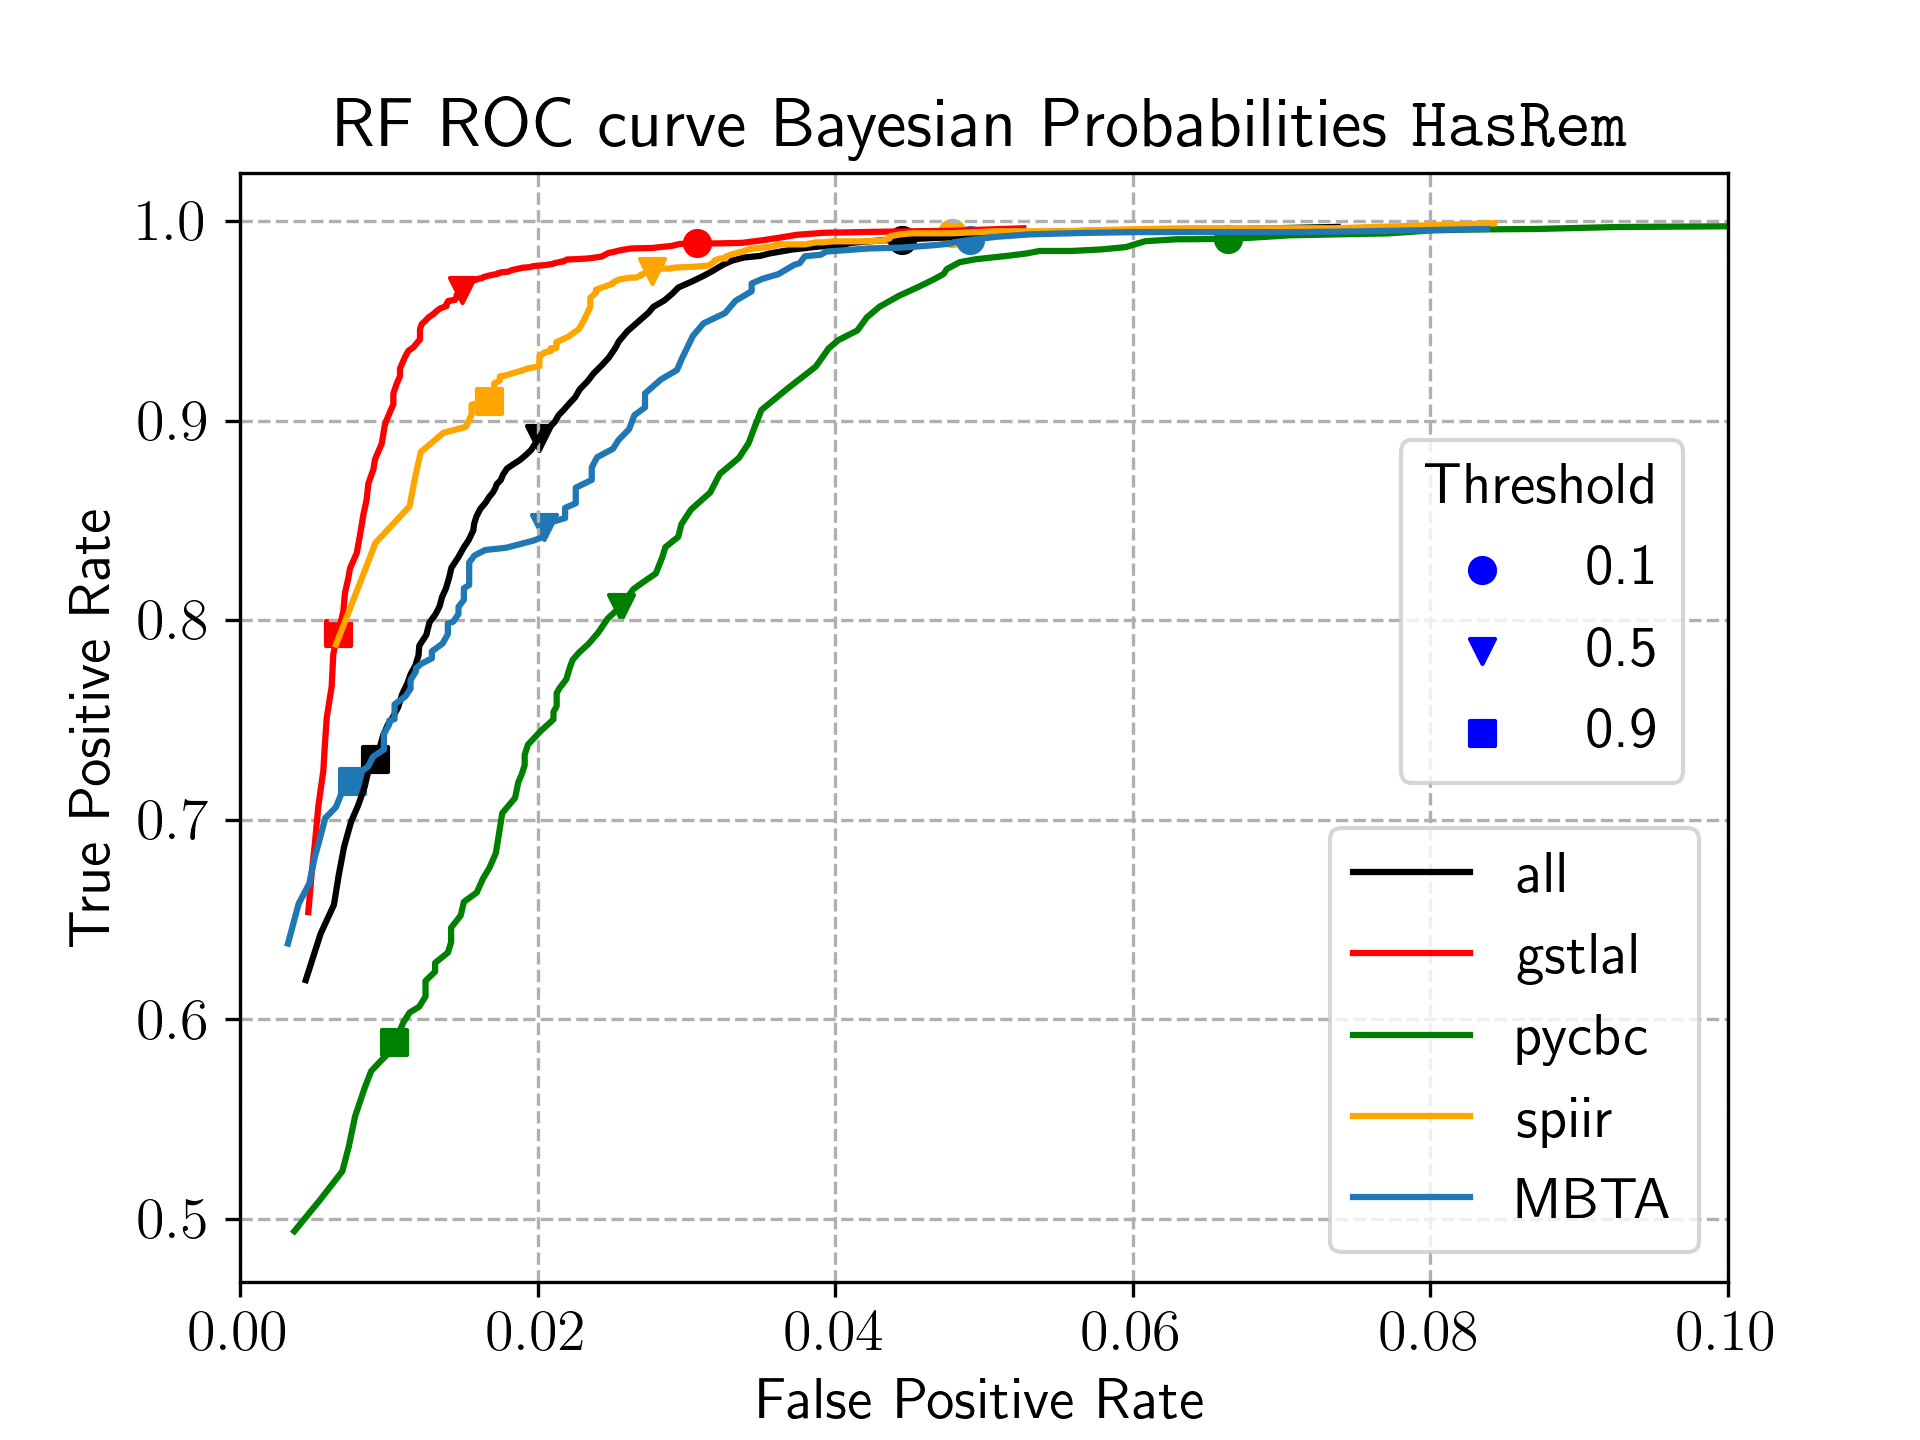
\includegraphics{RF_bayesian_REM}
\caption{\label{fig:rocMDC_KNN}ROC curves of Bayesian probability marginalized for the 23 EoSs for MDC11 dataset using \ac{RF} classifier.}
\end{figure}


Parameter sweeps (done, Miquel)


%Here are the results for the methods:

%\subsection{KNN Results}

%\mmt{We are only using 5 features, the independent variables: 
%\begin{equation*}
	%\big[m_1,m_2,\chi_1,\chi_2, \rm{SNR}\big]\,.
%\end{equation*}}

\subsubsection{\mmt{Has NS}}
\mmt{The metric we use to compute the distance between neighbors is the \textit{Manhattan} metric (or the Minkowski's $L1$ distance),  which is the distance between two points measured along axes at right angles. Having $p_1(x_1,y_1)$ and $p_2(x_2,y_2)$ the distance will be}
\begin{equation}
	d = |x_1-x_2|+|y_1-y_2|\,.
\end{equation}

\mmt{Moreover, the points are weighted uniformly.  After applying cross-validation,  we get that the optimal number of neighbors is $K_{\rm NS} = 10$, with a mean score $\rm{s_m} = 0:9718355224352762$ and a testing score  $\rm{s_t} = 0.9723828730478842$.} 

%\begin{figure}
%    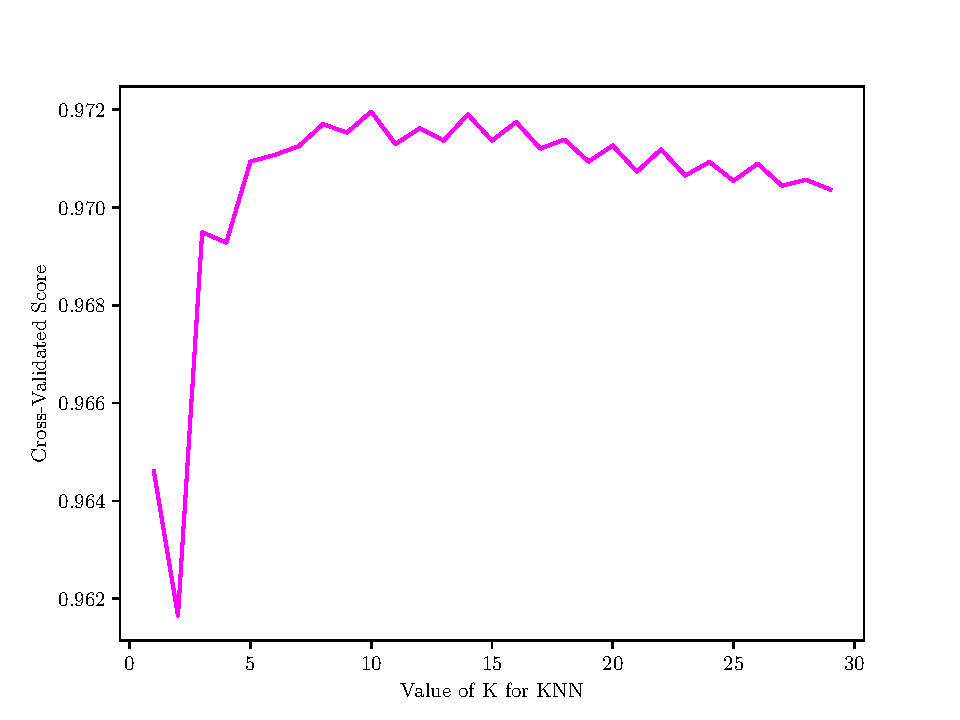
\includegraphics[width = 0.4\textwidth]{CrossValK.pdf}
%    \caption{Score of our KNN model as a function of the number of neighbors. We are considering \textit{HasNS}.}
%    \label{fig:crossvalK}
%\end{figure}
    
\begin{figure}
    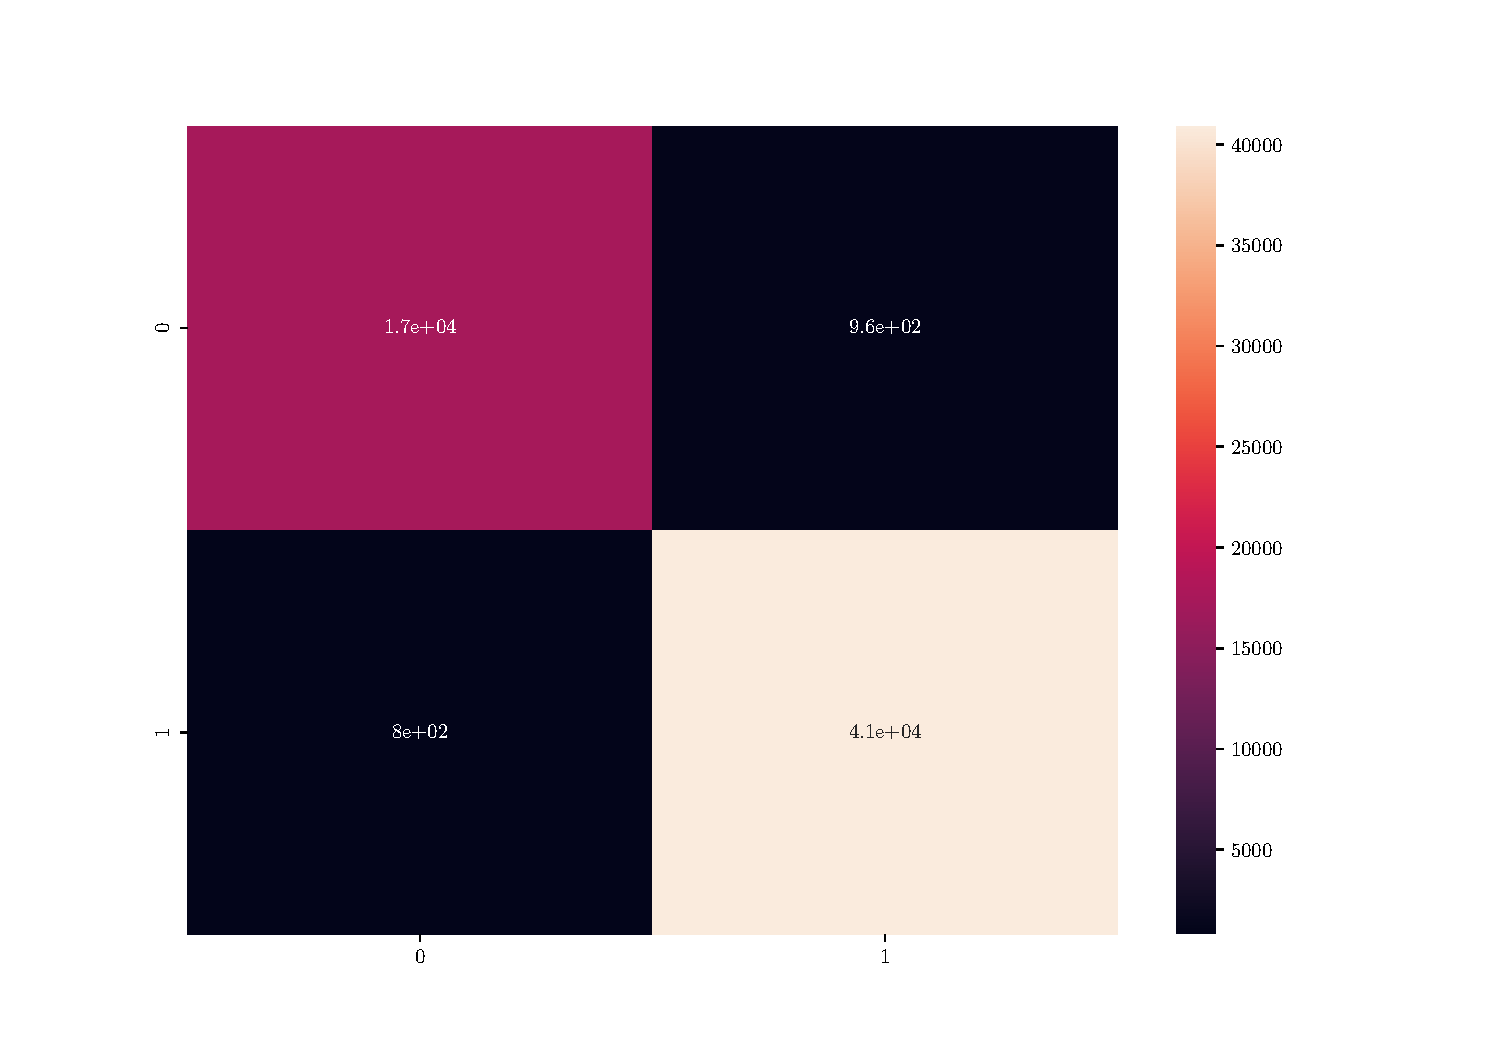
\includegraphics[width=0.45\textwidth]{figs/conf_matrix_NS.pdf}
    \caption{Confusion matrix for our model for \textit{HasNS}, using the independent recovered values. }
    \label{fig:confmat}
\end{figure}

\begin{figure}
    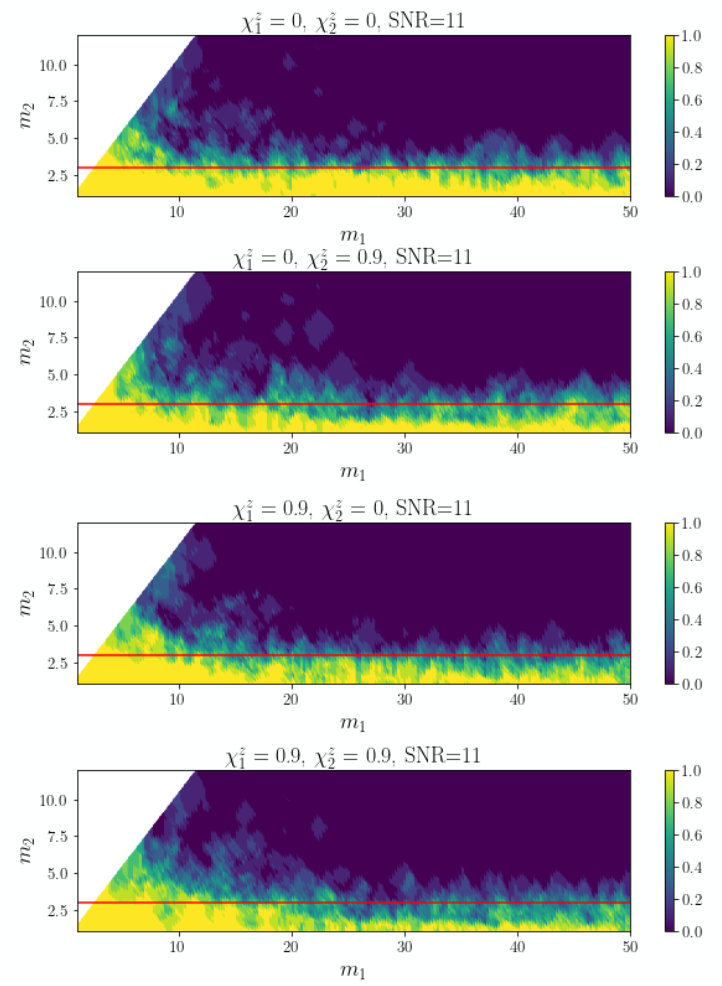
\includegraphics[width = 0.4\textwidth]{plot_fig4_chatt_spins.png}
  %   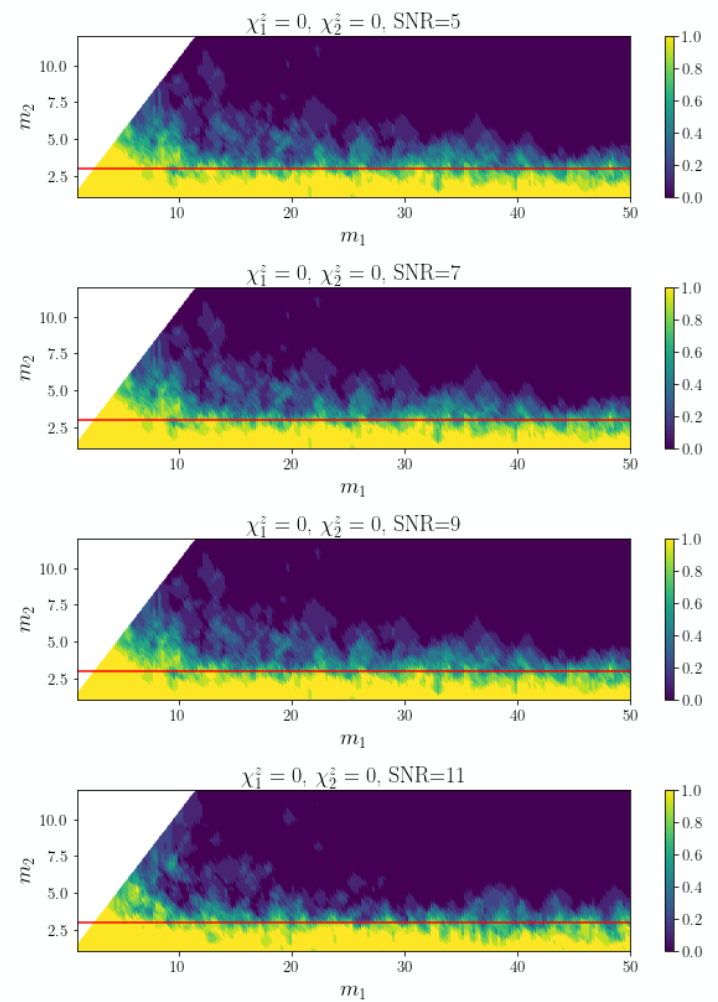
\includegraphics[width = 0.4\textwidth]{/Users/miquelmiravet/Projects/IPAM_LA/ML_group/IPAM2021_ML/algo/classy_KNN/PLOTS_KNN/NS_set/plots_miq/plot_fig4_chatt_snr.png}
    \caption{Probability of having a remnant as a function of the values of the masses. The different panels show the results for different spins. The solid red line depicts the threshold mass for $m_2$.}
    \label{fig:m1m2}
\end{figure}

\begin{figure}
	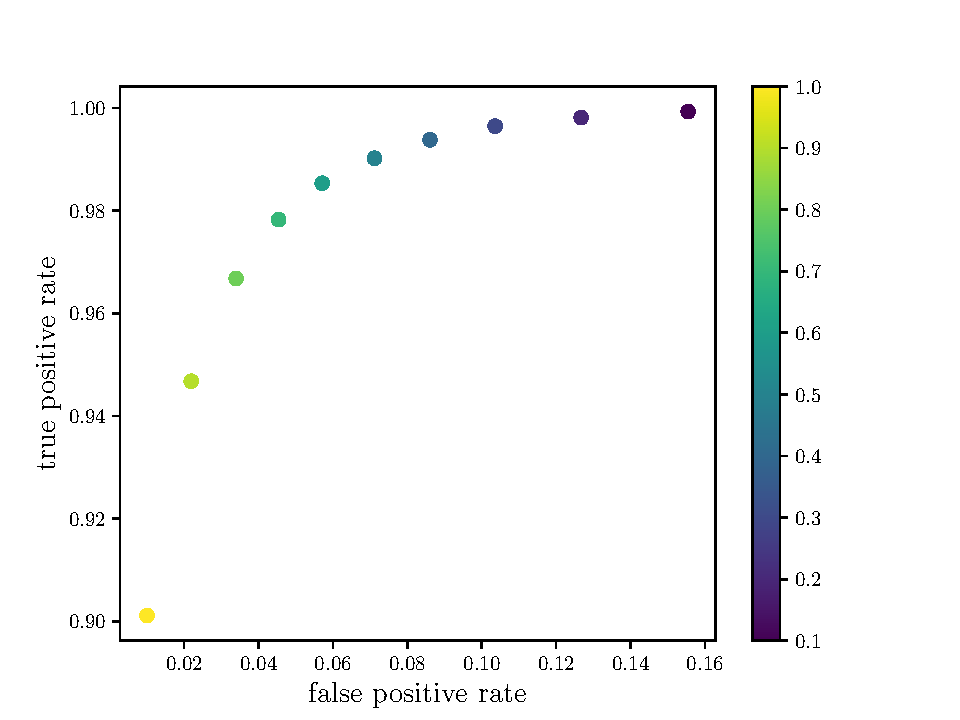
\includegraphics[width =0.4\textwidth]{ROCplot.pdf}
    \caption{Relation of the true and false positive rates as a function of the threshold applied to make the decision between having or not having a remnant. }
    \label{fig:roc}
\end{figure}

\mmt{In Fig.~\ref{fig:crossvalK} you can find how the mean score changes with the number of neighbors of the algorithm.  The confusion matrix appears in Fig.~\ref{fig:confmat}, the probability as a function of $m_1$ and $m_2$  is shown in Figs.~\ref{fig:m1m2}, and the true and false positive rates in terms of the threshold probability appear in Fig.~\ref{fig:roc}.}


 %plots and comments
%\subsection{RF Results}

We apply crossvalidation in the number of trees and depth of the forests for the 23 EoS, fixing the information gain criteria to \texttt{entropy}. We also save the second best option for comparison, and save both forests for each EoS in order to compare the file size. As the goal is to provide a model that can run in a low latency pipeline the amount of memory it can take is limited, even more when there will be 23 different model for the EoS generalization.

In table \ref{tab:RFcross} we present a summary of best and second best hyperparameters found in the crossvalidation for each EoS, along the memory the model occupies and the difference in the score. As we can see, usually a forest with many trees has a second best option with far less that is lighter in memory and achieves a similar performance. The optimum maximum depth is always 15. Also the score achieved for every EoS is similar, and so we check that our accuracy is not NS model dependent.

\begin{table*}[h]
\centering
\begin{tabular}{@{}lcccccccc@{}}
\toprule
                                & \multicolumn{4}{c}{Best}                                & \multicolumn{4}{c}{Second best}                            \\ \midrule
\multicolumn{1}{|l|}{EOS}       & Trees & Depth & Size(MB)    & \multicolumn{1}{c|}{Score}      & Trees & Depth & Size(MB)    & \multicolumn{1}{c|}{$\Delta$score} \\ \midrule
\multicolumn{1}{|l|}{APR4\_BB}  & 300   & 15    & 94.7  & \multicolumn{1}{c|}{0.9683018}  & 50    & 15    & 15.7  & \multicolumn{1}{c|}{3.35e-5}       \\ \midrule
\multicolumn{1}{|l|}{BHF\_BBB2} & 80    & 15    & 24.4  & \multicolumn{1}{c|}{0.9685127}  & 300   & 15    & 91.6  & \multicolumn{1}{c|}{5.16e-5}       \\ \midrule
\multicolumn{1}{|l|}{H4}        & 80    & 15    & 29.6  & \multicolumn{1}{c|}{0.9618587}  & 300   & 15    & 111.4 & \multicolumn{1}{c|}{1.19e-4}       \\ \midrule
\multicolumn{1}{|l|}{HQC18}     & 300   & 15    & 93.7  & \multicolumn{1}{c|}{0.9673755}  & 100   & 15    & 31.3  & \multicolumn{1}{c|}{3.06e-4}       \\ \midrule
\multicolumn{1}{|l|}{KDE0V}     & 300   & 15    & 92.0  & \multicolumn{1}{c|}{0.9673295}  & 80    & 15    & 24.5  & \multicolumn{1}{c|}{2.06e-4}       \\ \midrule
\multicolumn{1}{|l|}{KDE0V1}    & 100   & 15    & 30.9  & \multicolumn{1}{c|}{0.96704954} & 80    & 15    & 24.5  & \multicolumn{1}{c|}{3.43e-5}       \\ \midrule
\multicolumn{1}{|l|}{MPA1}      & 80    & 15    & 27.2  & \multicolumn{1}{c|}{0.96601225} & 300   & 15    & 102.1 & \multicolumn{1}{c|}{8.19e-5}       \\ \midrule
\multicolumn{1}{|l|}{MS1\_PP}   & 300   & 15    & 113.5 & \multicolumn{1}{c|}{0.96563534} & 80    & 15    & 30.2  & \multicolumn{1}{c|}{1.15e-4}       \\ \midrule
\multicolumn{1}{|l|}{MS1B\_PP}  & 300   & 15    & 114.2 & \multicolumn{1}{c|}{0.96555340} & 100   & 15    & 38.0  & \multicolumn{1}{c|}{1.97e-4}       \\ \midrule
\multicolumn{1}{|l|}{RS}        & 300   & 15    & 103.8 & \multicolumn{1}{c|}{0.96447350} & 80    & 15    & 27.6  & \multicolumn{1}{c|}{2.36e-4}       \\ \midrule
\multicolumn{1}{|l|}{SK255}     & 300   & 15    & 105.8 & \multicolumn{1}{c|}{0.96472405} & 100   & 15    & 35.5  & \multicolumn{1}{c|}{3.69e-4}       \\ \midrule
\multicolumn{1}{|l|}{SK272}     & 300   & 15    & 109.0 & \multicolumn{1}{c|}{0.96401816} & 100   & 15    & 36.4  & \multicolumn{1}{c|}{1.99e-4}       \\ \midrule
\multicolumn{1}{|l|}{SKI2}      & 50    & 15    & 18.8  & \multicolumn{1}{c|}{0.96242338} & 300   & 15    & 112.8 & \multicolumn{1}{c|}{8.37e-5}       \\ \midrule
\multicolumn{1}{|l|}{SKI3}      & 50    & 15    & 19.0  & \multicolumn{1}{c|}{0.96174537} & 100   & 15    & 38.1  & \multicolumn{1}{c|}{6.62e-5}       \\ \midrule
\multicolumn{1}{|l|}{SKI4}      & 300   & 15    & 100.6 & \multicolumn{1}{c|}{0.96598969} & 30    & 15    & 9.8   & \multicolumn{1}{c|}{8.37e-5}       \\ \midrule
\multicolumn{1}{|l|}{SKI5}      & 100   & 15    & 38.2  & \multicolumn{1}{c|}{0.96343381} & 80    & 15    & 30.4  & \multicolumn{1}{c|}{1.16e-4}       \\ \midrule
\multicolumn{1}{|l|}{SKI6}      & 300   & 15    & 101.7 & \multicolumn{1}{c|}{0.96586928} & 30    & 15    & 10.0  & \multicolumn{1}{c|}{2.17e-4}       \\ \midrule
\multicolumn{1}{|l|}{SKMP}      & 300   & 15    & 100.2 & \multicolumn{1}{c|}{0.96544567} & 80    & 15    & 26.9  & \multicolumn{1}{c|}{1.69e-4}       \\ \midrule
\multicolumn{1}{|l|}{SKOP}      & 100   & 15    & 32.3  & \multicolumn{1}{c|}{0.96610459} & 300   & 15    & 96.2  & \multicolumn{1}{c|}{6.85e-5}       \\ \midrule
\multicolumn{1}{|l|}{SLy}       & 80    & 15    & 25.3  & \multicolumn{1}{c|}{0.96728884} & 300   & 15    & 95.2  & \multicolumn{1}{c|}{8.49e-5}       \\ \midrule
\multicolumn{1}{|l|}{SLY2}      & 100   & 15    & 31.8  & \multicolumn{1}{c|}{0.96745868} & 80    & 15    & 25.4  & \multicolumn{1}{c|}{2.38e-4}       \\ \midrule
\multicolumn{1}{|l|}{SLY9}      & 300   & 15    & 101.6 & \multicolumn{1}{c|}{0.96605993} & 100   & 15    & 34.1  & \multicolumn{1}{c|}{1.51e-4}       \\ \midrule
SLY230A                         & 300   & 15    & 95.5  & 0.96714915                      & 100   & 15    & 31.9  & 2.53e-4                            \\ \bottomrule
\end{tabular}
\caption{Comparison of the best and second best RF models obtained during crossvalidation for all EoS. We show the file size in MB of the forest, and the difference in score between the two options.}
\label{tab:RFcross}
\end{table*}

To simplify the model and according to the results of crossvalidation, we train the final forests for all EoS with 50 trees and 15 maximum depth. In figure \ref{fig:RF_roc} we show the ROC curves for all models to give an idea of the performance. Notice that HasREM performs better than HasNS. The ourperformance of HasREM against HasNS in RF is even more noticeable in the histograms in figures \ref{fig:RF_hist_BHFBBB2}, \ref{fig:RF_hist_SLY} and \ref{fig:RF_hist_MS1PP} for the highlighted EoS, where the bars of asigned probabilities do not intersect each other and therefore there exists a threshold value for perfect classification in the testing dataset.

\begin{figure}
\centering
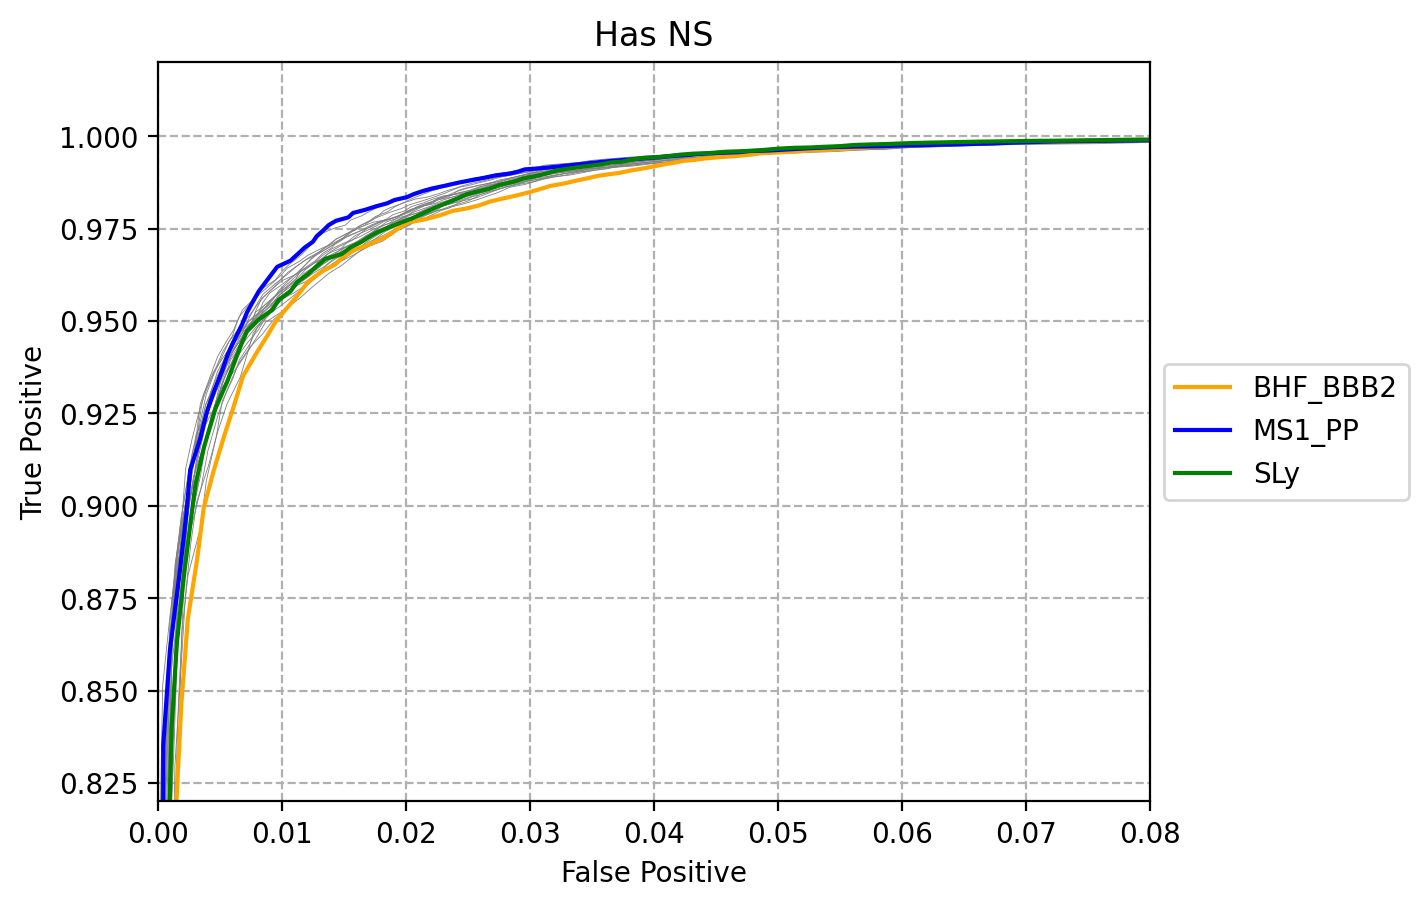
\includegraphics[width=0.45\textwidth]{/figs/HasNS_roc}
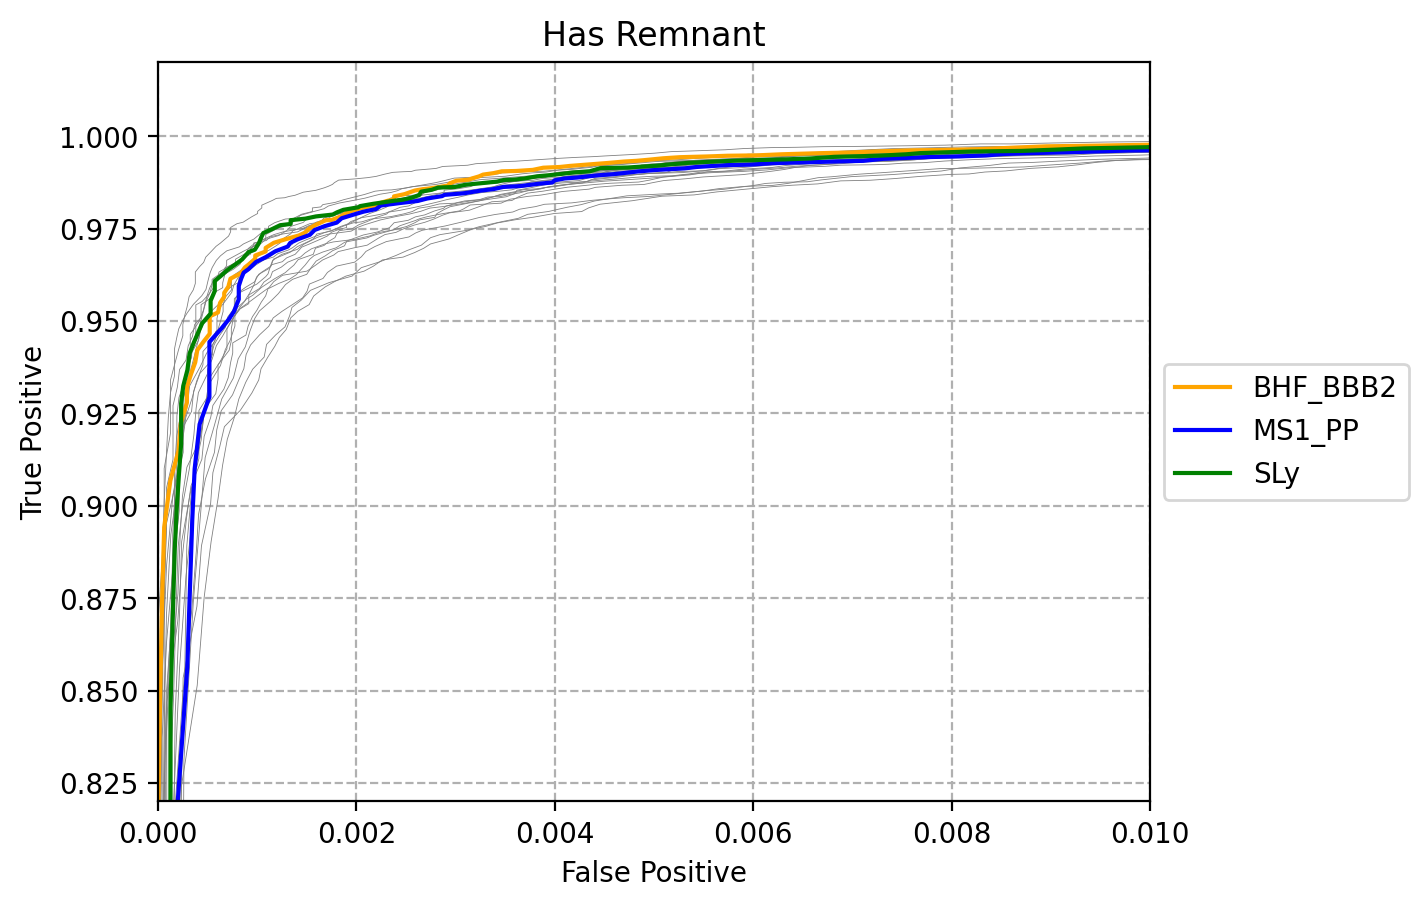
\includegraphics[width=0.45\textwidth]{/figs/HasREM_roc}
\caption{\label{fig:RF_roc} ROC curves}
\end{figure}

\begin{figure}
\centering
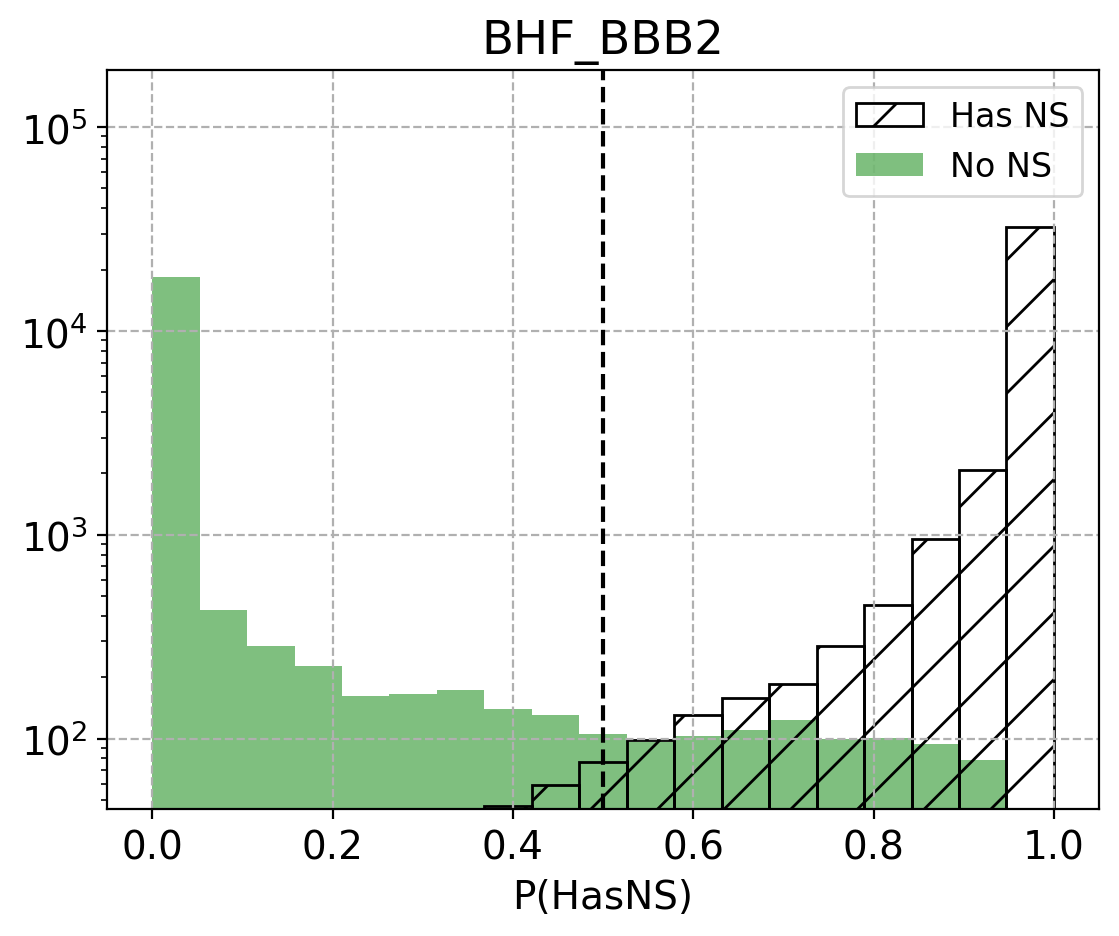
\includegraphics[width=0.45\textwidth]{/figs/BHF_BBB2_NShist}
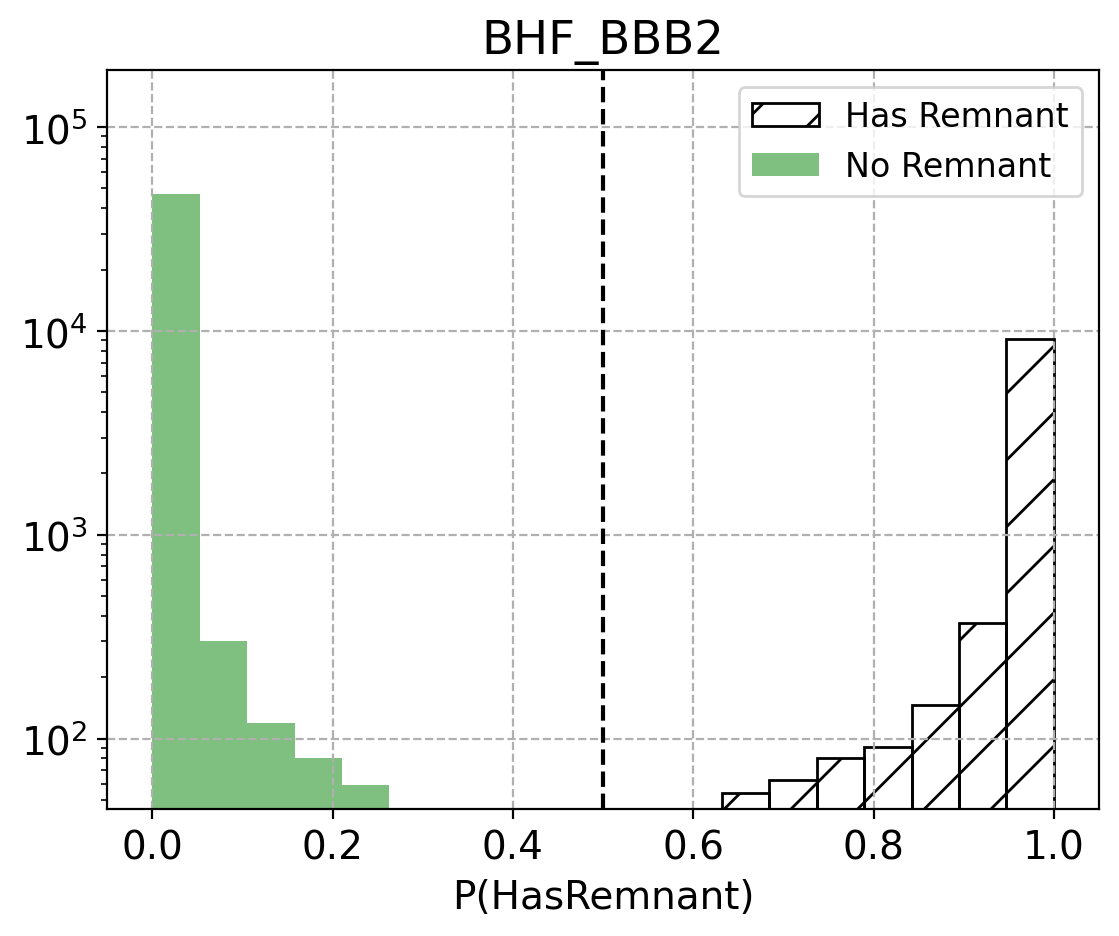
\includegraphics[width=0.45\textwidth]{/figs/BHF_BBB2_REMhist}
\caption{\label{fig:RF_hist_BHFBBB2} Histograms BHF BBB2}
\end{figure}

\begin{figure}
\centering
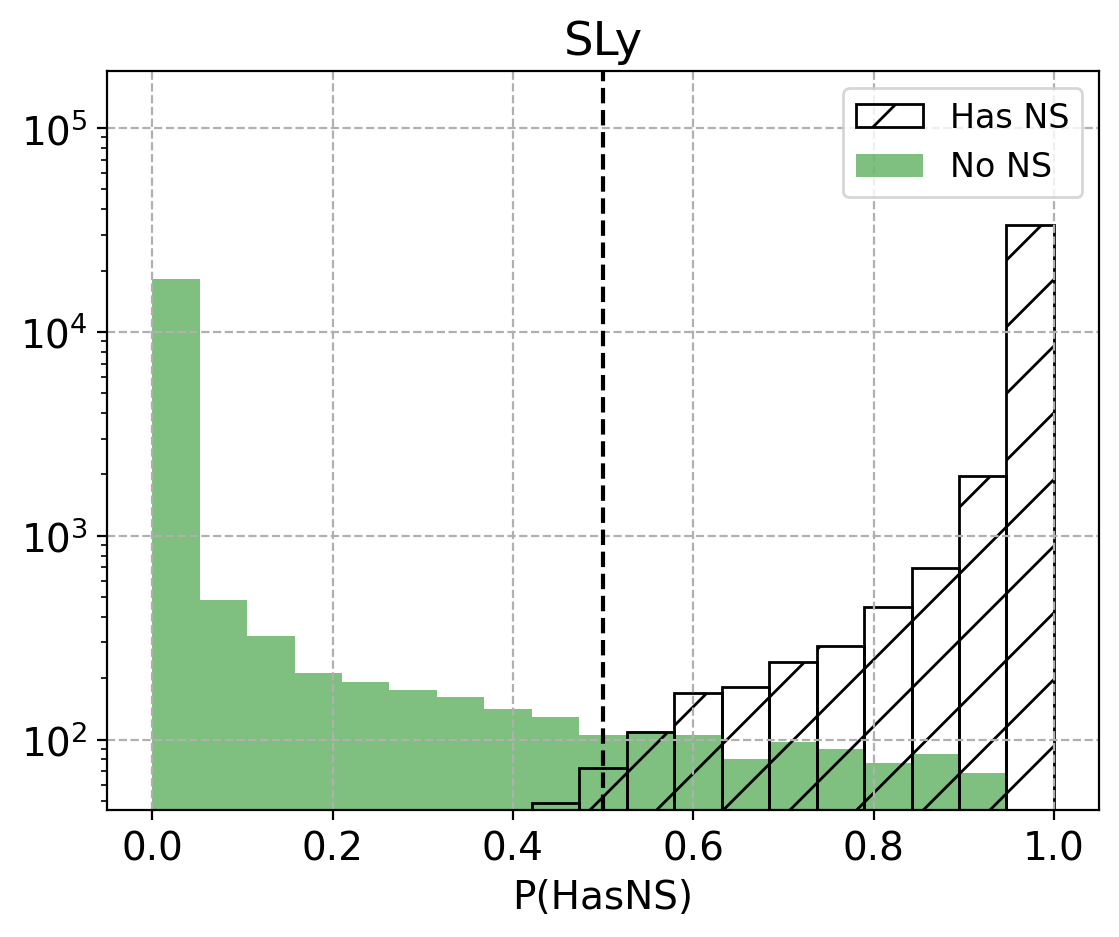
\includegraphics[width=0.45\textwidth]{/figs/SLy_NShist}
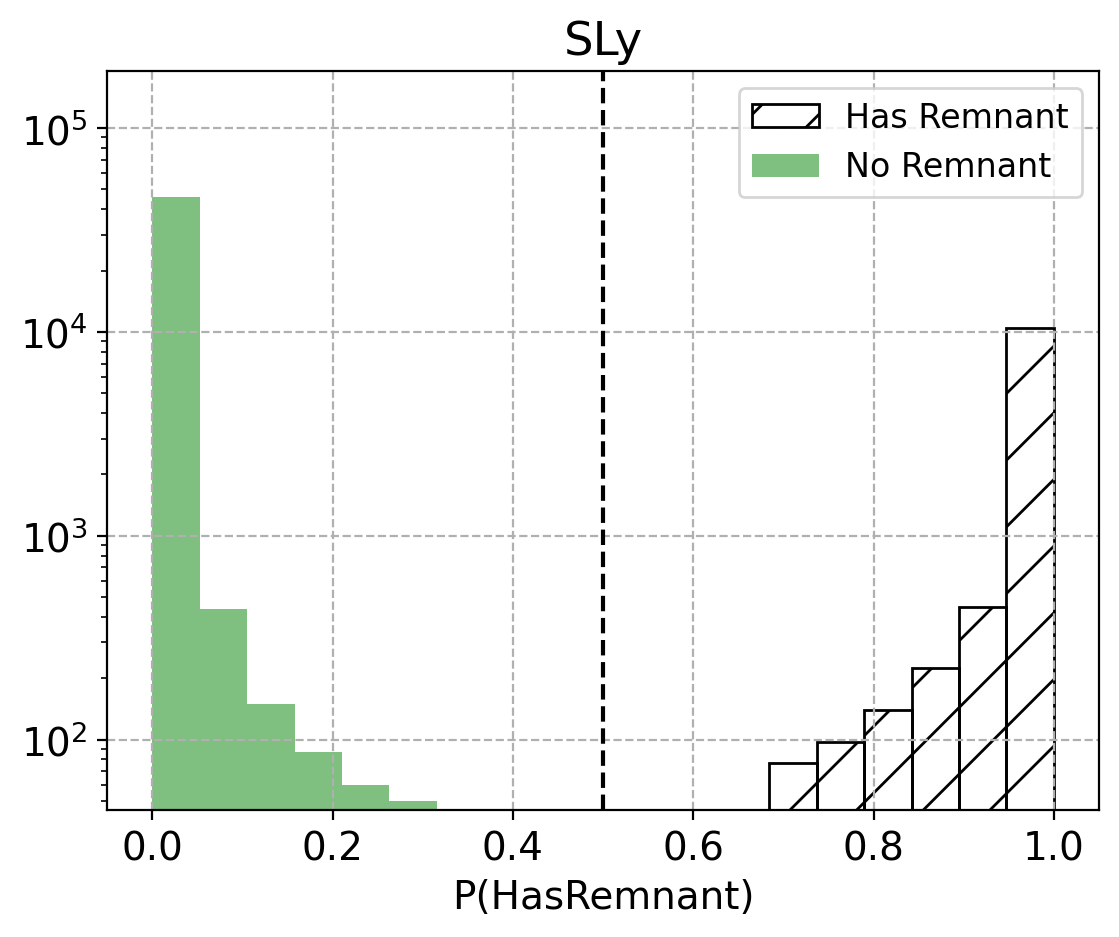
\includegraphics[width=0.45\textwidth]{/figs/SLy_REMhist}
\caption{\label{fig:RF_hist_SLY} Histograms SLy}
\end{figure}

\begin{figure}
\centering
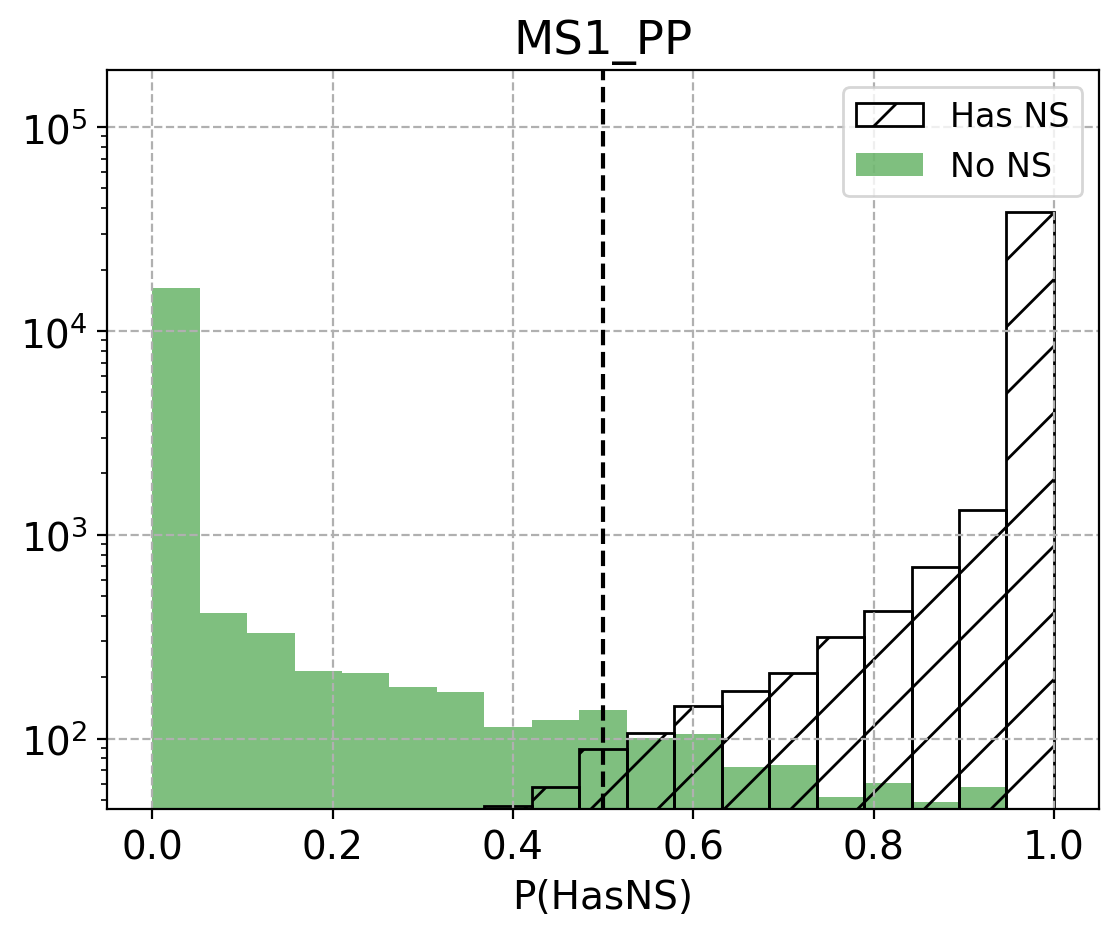
\includegraphics[width=0.45\textwidth]{/figs/MS1_PP_NShist}
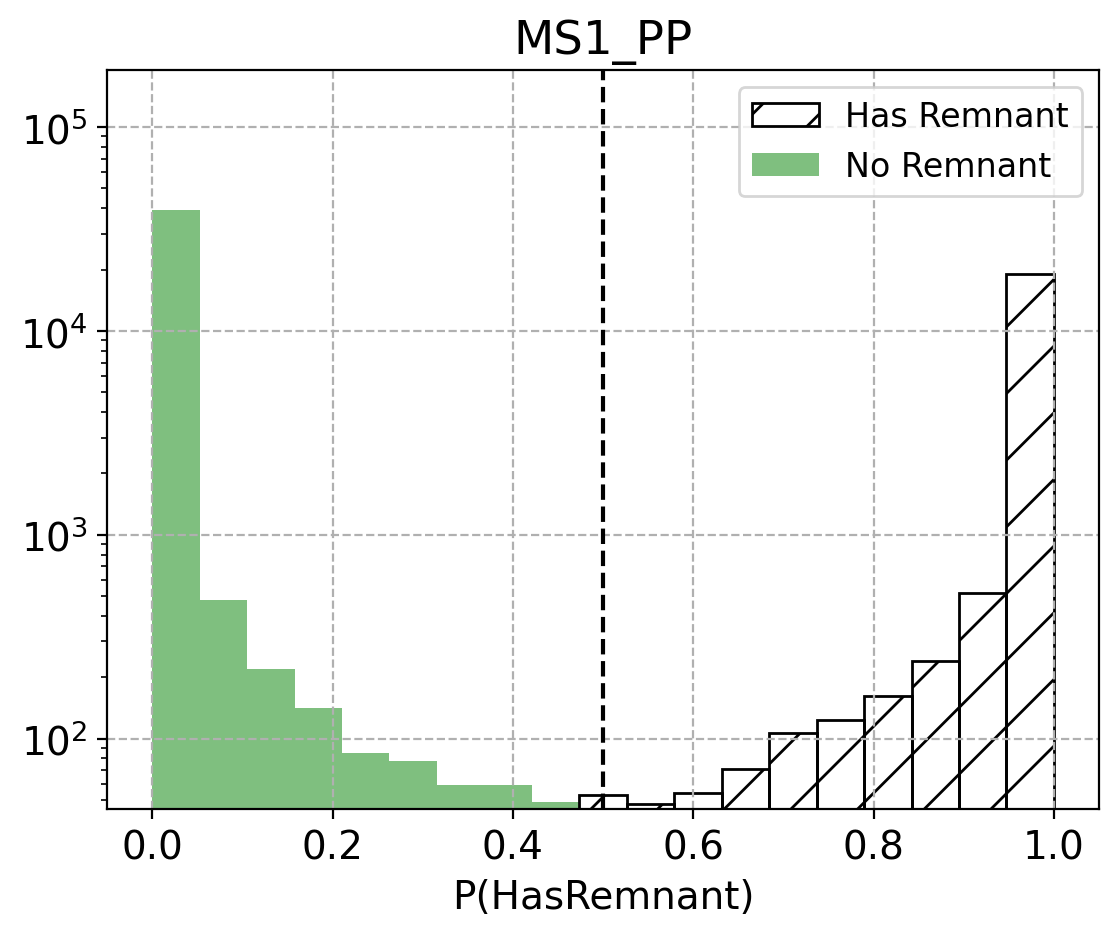
\includegraphics[width=0.45\textwidth]{/figs/MS1_PP_REMhist}
\caption{\label{fig:RF_hist_MS1PP} Histograms MS1 PP}
\end{figure}


 %plots and comments
%\input{GP_Results.tex}


In order to decide which method gives a better performance in classifying this kind of events, we can apply them over testing data and finally do a comparison between both. A way to see how data is classified we can construct histograms where the number of events that are classified with a label (\texttt{HasNS/HasRemnant}) \texttt{True} or \texttt{False} will change with a given threshold of the probability. For an algorithm with perfect performance, all the events with label \texttt{True (False)} should be at \textit{p}(\texttt{label}) = 1 (\textit{p}(\texttt{label}) = 0).

Another way to check the algorithm's performance is by building the so-called \textit{Receiver Operating Characteristic (ROC) Curve}. They show the variation of the true-positive rate (or efficiency) with the false-positive rate given a certain threshold for the probability. An algorithm with a proper performance will give a steeper ROC curve, or in other words, will have a higher eficiency with a lower false-positive rate.  


In the ROC curves that we will present in the following subsections, we highlight three reference EoS in color, from which we show results in more detail. We select BHF\_BBB2 because is the model that give the lowest maximum mass, MS1\_PP as the model with the bigger maximum mass, and we also include SLy because is the most accepted EoS for NS modeling (reference), and is the one that was used in the injections that are our dataset.


\subsection{Algorithm comparison}


%Here we talk about overall results and specifically from each algorithm in the
%subsections below.  \mmt{[MMT: Below I described how to check the performance of the algorithms. Maybe a table with all the scores/sensitivities/precisions from both %KNN and RF would be useful (already got it in a google doc)]}

%\mmt{To measure the performance of the classifiers we use some common statistical quantities.  The score is the number of correctly predicted events over the number %of total events (a perfect classifier has a score of 1).  It works best when there is an equal number of events for each label in the training set. It does not %consider the importance of misclassification, or that the training data can be biased towards one specific label.}

%\mmt{The mean score is computed by training the algorithm on the $90\%$ of the dataset and testing it on the remaining $10\%$, cycling the train/test combination over %the full dataset. To do that, we are going to use the training dataset, since it's the larger one.  In order to train and test the model and create the different %plots, we are going to use the training and testing files. }

%\mmt{Another useful quantity is the sensitivity. It is the ratio between the true positives and the sum of the true positives and false negatives.  It measures how %much the algorithm predicts \textit{true} (in our case it would be that the event has NS or has REM), when it is actually \textit{true}.Having a sensitivity equal to %1 would mean that our method predicts \textit{true} for every event. Therefore, a method with high sensitivity will barely miss true alarms. }

%\mmt{A quantity that measures how much you can trust a method when it predicts \textit{true} is the precision.  It is the ratio between the true positives and the %some of the true  and the false positives. A precision equal to 1 means that the method never predicts \textit{true} when it is actually \textit{false}. This means %that the method will never give false alarms. }

%\mmt{Finally, the F1 score $F1 = 2(\rm{precision \times sensitivity})/(\rm{precision+sensitivity})$ is a type of score that takes into consideration how precision and %sensitivity compensate each other. A perfect classifier would have a F1 score of 1.}

%To compare quantitatively the results from RF and KNN we compute the true positive and false positive rate for several threshold values, for both HasNS and HasREM, for the three selected EoS. These are tables \ref{tab:TPbhf}, \ref{tab:TPms1} and \ref{tab:TPsly}. For HasNS the two algorithms perform similarly, with almost the same TP for all threshold values and accross EoSs, although the false positive is smaller always in the RF. For HasREM we obtain that RF performs better than KNN in every case, with not only a smaller false positive rate, but a greater true positive rate.

%\begin{table}[]
%\centering
%\begin{tabular}{@{}c|cccc|cccc@{}}
%\toprule
%\multicolumn{1}{l|}{}          & \multicolumn{4}{c|}{Has NS}                       & \multicolumn{4}{c}{Has REM}                      \\ \midrule
%                               & \multicolumn{2}{c}{RF} & \multicolumn{2}{c|}{KNN} & \multicolumn{2}{c}{RF} & \multicolumn{2}{c}{KNN} \\
%\multicolumn{1}{l|}{Threshold} & TP         & FP        & TP          & FP         & TP         & FP        & TP         & FP         \\ \midrule
%0.1                            & 0.999      & 0.107     &   0.999          &  0.156          & 0.998      & 0.011     &    0.992        &  0.051          \\
%0.3                            & 0.998      & 0.068     &   0.996        &  0.117          & 0.993      & 0.005     &   0.974         &  0.017          \\
%0.5                            & 0.994      & 0.042     &   0.991          &  0.088           & 0.985      & 0.003     &   0.937         &  0.006          \\
%0.8                            & 0.967      & 0.014     &   0.966          & 0.043            & 0.957      & 0.001     &  0.845          &   0.001         \\ %\bottomrule
%\end{tabular}
%\caption{BHF\_BB2}
%\label{tab:TPbhf}
%\end{table}



\begin{table}[]
\begin{tabular}{c|c|ccr|ccr}
\hline
\multicolumn{1}{c|}{}         & \multicolumn{1}{l|}{} & \multicolumn{3}{c|}{p(HasNS)}                                                & \multicolumn{3}{c}{p(HasREM)}                                                \\ \hline
\multicolumn{1}{c|}{event ID} & grace\_id             & \multicolumn{1}{c}{RF} & \multicolumn{1}{c}{KNN} & \multicolumn{1}{c|}{GP} & \multicolumn{1}{c}{RF} & \multicolumn{1}{c}{KNN} & \multicolumn{1}{c|}{GP} \\ \hline
GW170823                      & G298936               & 0.000                   & 0.000                    & 0.014                   & 0.000                   & 0.000                    & 0.001                   \\
GW170817                      & G298048               & 1.000                   & 1.000                    & 0.999                   & 1.000                   & 1.000                    & 0.995                   \\
GW170814                      & G297595               & 0.000                   & 0.000                    & 0.013                   & 0.000                   & 0.000                    & 0.001                   \\
GW170809                      & G296853               & 0.002                   & 0.000                    & 0.013                   & 0.000                   & 0.000                    & 0.001                   \\
GW190408                      & G329243               & 0.000                   & 0.000                    & 0.013                   & 0.000                   & 0.000                    & 0.001                   \\
GW190412                      & G329483               & 0.000                   & 0.000                    & 0.021                   & 0.000                   & 0.000                    & 0.001                   \\
GW190413-052954               & G329577               & 0.000                   & 0.000                    & 0.013                   & 0.000                   & 0.000                    & 0.001                   \\
GW190413-134308               & G329615               & 0.000                   & 0.000                    & 0.010                   & 0.000                   & 0.000                    & 0.001                   \\
GW190421                      & G330300               & 0.000                   & 0.000                    & 0.017                   & 0.000                   & 0.000                    & 0.001                   \\
GW190425                      & G330564               & 1.000                   & 1.000                    & 0.999                   & 0.999                   & 1.000                    & 0.994                   \\
GW190426                      & G330687               & 0.996                   & 1.000                    & 0.980                   & 0.009                   & 0.000                    & 0.008                   \\
GW190503                      & G331315               & 0.000                   & 0.000                    & 0.032                   & 0.000                   & 0.000                    & 0.001                   \\
GW190512                      & G332169               & 0.000                   & 0.000                    & 0.014                   & 0.000                   & 0.000                    & 0.001                   \\
GW190513                      & G332333               & 0.000                   & 0.000                    & 0.014                   & 0.000                   & 0.000                    & 0.001                   \\
GW190517                      & G333132               & 0.000                   & 0.000                    & 0.010                   & 0.000                   & 0.000                    & 0.001                   \\
GW190519                      & G333443               & 0.000                   & 0.000                    & 0.014                   & 0.000                   & 0.000                    & 0.001                   \\
GW190521-074359               & G333664               & 0.000                   & 0.000                    & 0.013                   & 0.000                   & 0.000                    & 0.001                   \\
GW190602                      & G335015               & 0.000                   & 0.000                    & 0.061                   & 0.000                   & 0.000                    & 0.001                   \\
GW190630                      & G337426               & 0.000                   & 0.000                    & 0.014                   & 0.000                   & 0.000                    & 0.001                   \\
GW190706                      & G337919               & 0.015                   & 0.000                    & 0.019                   & 0.000                   & 0.000                    & 0.001                   \\
GW190707                      & G337978               & 0.000                   & 0.000                    & 0.096                   & 0.000                   & 0.000                    & 0.001                   \\
GW190708                      & G338125               & 0.000                   & 0.002                    & 0.070                   & 0.000                   & 0.000                    & 0.001                   \\
GW190720                      & G344653               & 0.004                   & 0.000                    & 0.024                   & 0.000                   & 0.000                    & 0.001                   \\
GW190727                      & G345173               & 0.011                   & 0.000                    & 0.013                   & 0.000                   & 0.000                    & 0.001                   \\
GW190728                      & G345315               & 0.000                   & 0.000                    & 0.013                   & 0.000                   & 0.000                    & 0.001                   \\
GW190814                      & G347305               & 0.098                   & 0.647                    & 0.878                   & 0.000                   & 0.000                    & 0.002                   \\
GW190828-063405               & G348500               & 0.002                   & 0.000                    & 0.014                   & 0.000                   & 0.000                    & 0.001                   \\
GW190828-065509               & G348519               & 0.001                   & 0.000                    & 0.019                   & 0.000                   & 0.000                    & 0.001                   \\
GW190915                      & G350491               & 0.000                   & 0.000                    & 0.009                   & 0.000                   & 0.000                    & 0.001                   \\
GW190924                      & G351423               & 0.037                   & 0.075                    & 0.100                   & 0.000                   & 0.000                    & 0.001                   \\
GW190930                      & G351993               & 0.000                   & 0.000                    & 0.079                   & 0.000                   & 0.000                    & 0.001                   \\
GW191109                      & G354231               & 0.000                   & 0.000                    & 0.036                   & 0.000                   & 0.000                    & 0.001                   \\
GW191129                      & G355916               & 0.004                   & 0.000                    & 0.024                   & 0.000                   & 0.000                    & 0.001                   \\
GW191204-171526               & G356500               & 0.000                   & 0.000                    & 0.026                   & 0.000                   & 0.000                    & 0.001                   \\
GW191215                      & G357403               & 0.000                   & 0.000                    & 0.017                   & 0.000                   & 0.000                    & 0.001                   \\
GW191216                      & G357490               & 0.000                   & 0.000                    & 0.125                   & 0.000                   & 0.000                    & 0.001                   \\
GW191222                      & G358088               & 0.000                   & 0.000                    & 0.028                   & 0.000                   & 0.000                    & 0.001                   \\
GW200112                      & G359994               & 0.000                   & 0.000                    & 0.015                   & 0.000                   & 0.000                    & 0.001                   \\
GW200115                      & G360364               & 0.997                   & 1.000                    & 0.987                   & 1.000                   & 0.000                    & 0.011                   \\
GW200129                      & G361581               & 0.000                   & 0.000                    & 0.015                   & 0.000                   & 0.000                    & 0.001                   \\
GW200219                      & G364596               & 0.000                   & 0.000                    & 0.027                   & 0.000                   & 0.000                    & 0.001                   \\
GW200224                      & G365371               & 0.014                   & 0.000                    & 0.027                   & 0.000                   & 0.000                    & 0.001                   \\
GW200225                      & G365427               & 0.001                   & 0.000                    & 0.013                   & 0.000                   & 0.000                    & 0.001                   \\
GW200302                      & G366190               & 0.000                   & 0.000                    & 0.014                   & 0.000                   & 0.000                    & 0.001                   \\
GW200311                      & G367788               & 0.000                   & 0.000                    & 0.01                    & 0.000                   & 0.000                    & 0.001                   \\
GW200316                      & G368545               & 0.000                   & 0.000                    & 0.068                   & 0.000                   & 0.000                    & 0.001                   \\
GW200322                      & G369200               & 0.012                   & 0.000                    & 0.031                   & 0.000                   & 0.000                    & 0.001                   \\ \cline{1-1} \cline{3-4} \cline{6-7}
\hline
\end{tabular}
\caption{PROBAB TABLE REAL DATA - from algo. Update to marginalized bayesian or remove.}
\label{tab:real_data}
\end{table}



\begin{table}[]
\begin{tabular}{c|c|cc|cc}
\hline
\multicolumn{1}{c|}{}         & \multicolumn{1}{l|}{} & \multicolumn{2}{c|}{p(HasNS)}                                                & \multicolumn{2}{c}{p(HasREM)}                                                \\ \hline
\multicolumn{1}{c|}{event ID} & grace\_id             & \multicolumn{1}{c}{RF} & \multicolumn{1}{c}{KNN}  & \multicolumn{1}{c}{RF} & \multicolumn{1}{c}{KNN} \\ \hline
GW170817                      & G298048               & 1.000                   & 1.000                    & 1.000                   & 1.000                                  \\
GW190425                      & G330564               & 1.000                   & 1.000                    & 0.999                   & 1.000                             \\
GW190426                      & G330687               & 0.996                   & 1.000                    & 0.009                   & 0.000                     \\
GW190814                      & G347305               & 0.098                   & 0.647                    & 0.000                   & 0.000                      \\
GW190924                      & G351423               & 0.037                   & 0.075                    & 0.000                   & 0.000                       \\               
GW200115                      & G360364               & 0.997                   & 0.987                   & 0.006                   & 0.000                           \\
\hline
\end{tabular}
\caption{Short table with probabilities (from algo) for O3 real events. I don't think we want this anymore.}
\label{tab:real_data_short}
\end{table}

\begin{table}[]
\begin{tabular}{c|c|cc|cc}
\hline
\multicolumn{1}{c|}{}         & \multicolumn{1}{l|}{} & \multicolumn{2}{c|}{p(HasNS)}                                                & \multicolumn{2}{c}{p(HasREM)}                                                \\ \hline
\multicolumn{1}{c|}{event ID} & grace\_id             & \multicolumn{1}{c}{RF} & \multicolumn{1}{c}{KNN}  & \multicolumn{1}{c}{RF} & \multicolumn{1}{c}{KNN} \\ \hline
GW170817                      & G298048               & 0.9977                   & 0.9885                    & 0.9970                   & 0.9847                                  \\
GW190425                      & G330564               & 0.9977                   & 0.9885                    & 0.9969                   & 0.9847                             \\
GW190426                      & G330687               & 0.9971                   & 0.9847                    & 0.0003                   & 0.0                     \\
GW190814                      & G347305               & 0.0418                   & 0.5665                   & 0.0                  & 0.0                      \\
GW190924                      & G351423               & 0.0122                   & 0.0536                   & 0.0                   & 0.0                       \\               
GW200115                      & G360364               & 0.9976                   & 0.9885                   & 0.0                  & 0.0                           \\
\hline
\end{tabular}
\caption{Short table with BAYESIAN probabilities for O3 real events. Marginalized, right?}
\label{tab:real_data_bayesian}
\end{table}


%comparing both, TP and FP and what do we think


\section{Conclusions\label{conclusions}}

In this paper, we have presented a new scheme for real-time classification of \ac{GW} \ac{CBC} signals detected by the \ac{LVK} detectors. The method uses the output of the \ac{LVK}
low-latency pipelines to identify whether the GW source progenitor contains a \ac{NS} (\hasns) and a post-merger matter remnant is produced in the merger (\hasrem). Estimates of these
metrics are included in public alerts for candidate \ac{GW} events issued by the \ac{LVK}. Determining these metrics in low latency is crucial to enabling coincident \ac{MMA} observations
of GW and \ac{EM} signatures.

We have assessed the viability and measured the performance of two classifiers, \ac{KNN} and \ac{RF}, on two sets of real detector data augmented with synthetic GW injections of GW
signals that were generated for space-time volume sensitivity analyses of \ac{O2} \ac{LVK} \ac{GW} searches~\cite{Chatterjee:2019avs} and an \ac{MDC} real-time replay of \ac{O3}
data~\cite{Chaudhary:2023vec}. 


One important novel ingredient of the proposed scheme is the computation of Bayesian probabilities for \hasns\ and \hasrem. Until now, the information that has been passed to astronomers
in public alerts has been in the form of binary classification scores for these metrics. Here, we provide a method to compute \hasns\ and \hasrem\ as actual probabilities that the \ac{GW}
source includes a neutron star and post-merger matter remnant. Therefore, our scheme provides more direct and easily interpretable information to aid the community of astronomers in
deciding whether to follow up on \ac{GW} candidate events with \ac{EM} observatories.

To construct the Bayesian probabilities for \hasns\ and \hasrem, we train and test the classifiers on the \ac{O2} data set following the customary 70\% -- 30\% split between training and
testing data. After evaluating the performance of the classifiers with standard \ac{ROC} curves, we use the testing set to generate numerical Bayesian probability expressions for the
models. This minimizes potential bias that may result from the use of data sets with different properties while ensuring that the Bayesian fits are built with data that is independent of the data used for training the classifiers. The effectiveness of the Bayesian fits is then evaluated on fully independent data sets using the \ac{O3} set and real detections. 

\tocheck{As shown in Appendix~\ref{app:comparison}, \sout{when tested on the (GstLAL-only) \ac{O2} set of recovered injections both our methods outperform the specific \ac{KNN} algorithm implementation that is currently used in the \ac{LVK} low-latency infrastructure when tested on the (GstLAL-only) \ac{O2} set
of recovered injections, with \ac{RF} outperforming \ac{KNN} for both \hasns\ and \hasrem.} our \ac{RF} implementation outperforms the specific \ac{KNN} algorithm implementation that is currently used in the \ac{LVK} low-latency infrastructure, and our \ac{KNN} approach performs similarly. }When tested on the \ac{O3} set, both algorithms improve on \hasns\ while underperforming on
\hasrem.  In this case, \ac{KNN} outperforms \ac{RF}, which exhibits more variation across different pipelines.  If only the injections recovered by GstLAL are considered in \ac{O3}, the
\ac{O3} results of both \ac{RF} and \ac{KNN} are consistent with \ac{O2}. \ac{RF}'s performance on \ac{O3} events recovered by other pipelines, on the other hand, is noticeably lower.
This appears to imply that \ac{RF} is less portable than \ac{KNN} across different data sets and pipelines. The different ways \ac{RF} and \ac{KNN} operate, as well as the different
characteristics of the sets, may explain their behavior.

The RF classifier is a decision tree-based classifier that sets decision rules by implementing specific cuts (conditions) on input features. The \ac{KNN} algorithm implements decision
rules by computing the nearest neighbors of input features in the parameter space for the data point of interest. \ac{RF} is designed to construct hard boundaries based on input
parameters, whereas the \ac{KNN} algorithm is designed to produce an outcome based on differences between features. As a result, the \ac{RF} algorithm's nature may make it more suitable
for classifying events with \hasns, which is based on a well-defined, hard boundary between positive and negative outcomes, such as the secondary mass value. To distinguish between
systems with zero and nonzero post-remnant matter in \hasrem, the algorithms must learn Foucart's fit from the recovered parameters. Foucart's formula is dependent on the \ac{EOS} under
consideration, as well as the pipeline that recovers the injection. Because \ac{RF} and \ac{KNN} are trained on injections that are only recovered by GstLAL, \ac{RF} is more affected than
\ac{KNN}. \tocheck{However, a comprehensive evaluation, involving datasets from new observing runs and diverse pipelines, would be needed to assert that \ac{KNN} is more flexible than \ac{RF}.}

This work provides an improved scheme to implement Bayesian probabilities for \hasns\ and \hasrem\ classification of candidate events that would be straightforward to deploy in the
existing LVK infrastructure. Our method can also be easily extended to other properties of \ac{GW} signals that are being or may be released in low latency, such as \hasgap\ among other
data products. Other future extensions of this work include improving algorithm training and Bayesian fit estimation with updated data sets of simulated injections in \ac{LVK} \ac{O4}
data generated with different pipelines and with better coverage of the mass gap region than the \ac{O2} data set. It would also be worthwhile to investigate the use of additional ML
classifiers that could further improve the process's accuracy, reduce the need for computational resources, and decrease latency. Finally, a similar infrastructure could be designed and
deployed to aid in the rapid parameter estimation of pipeline outputs, but with a focus on feature regression rather than classification. This latter line of investigation will be
presented in a future publication.




\section*{Acknowledgments}

We are very grateful to the authors of Ref.~\cite{Chatterjee:2019avs} for fruitful discussions and for sharing their work that helped us to directly compare our methods to those used in
\ac{LVK}'s \ac{O3} observing run. We would also like to thank the many other colleagues of the LIGO Scientific Collaboration and the Virgo Collaboration who have provided invaluable help
over the years and, in partcular, Tito Dal Canton, Thomas Dent, and Shaon Ghosh for their useful comments during the internal \ac{LVK} review period.

This work is based upon work supported by the LIGO Laboratory which is a major facility fully funded by the National Science Foundation. We are grateful for computational resources
provided by the LIGO Laboratory and supported by the U.S.\ National Science Foundation Awards PHY-0757058 and PHY-0823459. 

M.B.\ is partiallly supported by the Spanish Agencia Estatal de Investigaci\'on grant PID2020-118236GB-I00. M.M.T.\ is partially supported by the Ministerio de Universidades de Espa\~na
(Spanish Ministry of Universities) through the ``Ayuda para la Formaci\'on de Profesorado Universitario'' (FPU) grant FPU19/01750, by the Spanish Agencia Estatal de Investigaci\'on grants
PGC2018-095984-B-I00 and PID2021-125485NB-C21 funded by MCIN/AEI/10.13039/501100011033 and the European Regional Development Fund (ERDF) ``A way of making Europe,'' and by the Generalitat
Valenciana (Prometeo grant CIPROM/2022/49). S.S.C.\ and Y.Z.\ are partially supported by the U.S.\ National Science Foundation under awards PHY-2011334 and PHY-2308693. M.C.\ is partially
supported by the U.S.\ National Science Foundation under awards PHY-2011334, PHY-2219212 and PHY-2308693. L.M.Z.\ is partially supported by the MSSGC Graduate Research Fellowship, awarded
through the NASA Cooperative Agreement 80NSSC20M0101. D.T.~is partially supported by the Spanish Agencia Estatal de Investigaci\'on grant PID2021-125485NB-C21 funded by
MCIN/AEI/10.13039/501100011033 and ERDF ``A way of making Europe,'' and by the Generalitat Valenciana (Prometeo grant CIPROM/2022/49).

M.W.C.\ acknowledges support from the National Science Foundation with grant numbers PHY-2308862 and OAC-2117997. A.T.\ acknowledges support from the National Science Foundation with
grant numbers PHY-2010970 and OAC-2117997.

This research was initiated by M.B, M.M.T., S.A., M.C., L.M.Z., D.T., and Y.Z.\ during their stay at the Institute of Pure and Applied Mathematics (IPAM),  University of California
Los-Angeles (UCLA). IPAM is partially supported by the National Science Foundation through award DMS-1925919. These authors would like to thank IPAM and UCLA for their warm hospitality.

Software for this analysis is written in \texttt{Python} 3.x~\cite{python3} and uses standard Open Source libraries and community-contributed modules from the Python Package Index (PyPI)
repository~\cite{pypi} including \texttt{numpy}~\cite{harris2020array}, \texttt{scipy}~\cite{2020SciPy-NMeth}, \texttt{pandas}~\cite{reback2020pandas,mckinney-proc-scipy-2010},
\texttt{matplotlib}~\cite{Hunter:2007ouj}, and \texttt{sklearn}~\cite{scikit-learn}.

This manuscript has been assigned LIGO Document Control Center number P2300338.

\textbf{Author contribution statement.} M.B.\ and M.M.T.\ designed the \ac{RF} and \ac{KNN} models and their computational framework, respectively, and ran the corresponding analyses.
S.S.C.\ curated the data sets and contributed to the analysis, particularly the comparison with the current \ac{LVK} \ac{KNN} implementation. M.C.\ directed the project. S.A., L.M.Z.,
D.T., and Y.Z.\ contributed to all aspects of this work, including but not limited to the design and implementation of the research, data analysis, and manuscript writing.  Authorship for
the \ac{LVK} members of the \ac{MDC} builder's list is requested in publications resulting from the \ac{MDC} data set.  M.W.C.\ and A.T.\ are opt-in members of this list. M.W.C.\ also
provided some comments during the internal \ac{LVK} review period. The authors gratefully thank the other opt-out members of the \ac{MDC} builder's list for creating the set, and/or
providing summary statistics based on its results, and making these products available to the \ac{LVK} collaborations: Sarah Antier, Patrick J.~Brockill, Deep Chatterjee, Reed Essick,
Shaon Ghosh, Patrick Godwin, Erik Katsavounidis, and Gaurav Waratkar.








%\def\bibsection{\section*{References}}
%\bibliographystyle{aps}
\bibliography{classification}

\end{document}

% Local Variables: 
% mode: latex
% End:
